\chapter{Ρομποτική Πλατφόρμα} \label{Chapter2}

%----------------------------------------------------------------------------------------
%	SECTION 1: Monstertruck Robotic Platform
%----------------------------------------------------------------------------------------
\section{Ρομποτική Πλατφόρμα {Monstertruck}} \label{sec:robotic_platform}
Η ρομποτική πλατφόρμα {Monstertruck} αποτελεί ένα ρομποτικό όχημα, η ανάπτυξη του οποίου, ξεκίνησε στα πλαίσια της ομάδας P.A.N.D.O.R.A. και ολοκληρώθηκε στα πλαίσια της παρούσας διπλωματικής εργασίας. Αναπτύχθηκε με σκοπό την χρήση σε εφαρμογές αυτόνομων ρομποτικών οχημάτων, για χαρτογράφηση και εξερεύνηση άγνωστων περιβαλλόντων και αναζήτηση σημείων ενδιαφέροντος, αλλά ταυτόχρονα και για πειραματισμό με εναλλακτικά μοντέλα κίνησης οχημάτων.

\subsection{Τηλεκατευθυνόμενο Όχημα GroundPounder} \label{ssec:groundpounder}
Για την κατασκευή της ρομποτικής πλατφόρμας, χρησιμοποιήθηκε, σαν βάση, το τηλεκατευθυνόμενο όχημα GroundPounder της Redcat Racing. Ανήκει στην κατηγορία φορτηγών οχημάτων Monstertruck, με κλίμακα 1:10 και περιλαμβάνει σκελετό από αλουμίνιο, αναρτήσεις και σύστημα ανεξάρτητης στρέψης των μπροστινών και πίσω τροχών (Τετραδιεύθυνση ή 4-Wheel-Steering), σε συνδυασμό με μετάδοση της κίνησης και στους τέσσερις τροχούς ({Τετρακίνηση} ή {4-Wheel-Drive}), προσφέροντας μεγαλύτερη ευελιξία και δυνατότητες, συγκριτικά με τα συμβατικά αυτοκίνητα, που περιλαμβάνουν στρέψη, μόνο, των μπροστινών τροχών ({Μπροστινοδιεύθυνση ή Front-Wheel-Steering}) και κίνηση μόνο των μπροστινών ({Μπροστινοκίνηση ή Front-Wheel-Drive}) ή μόνο των πίσω τροχών ({Πισωκίνηση ή Rear-Wheel-Drive}).

\begin{figure}[!ht]
	\begin{center}
		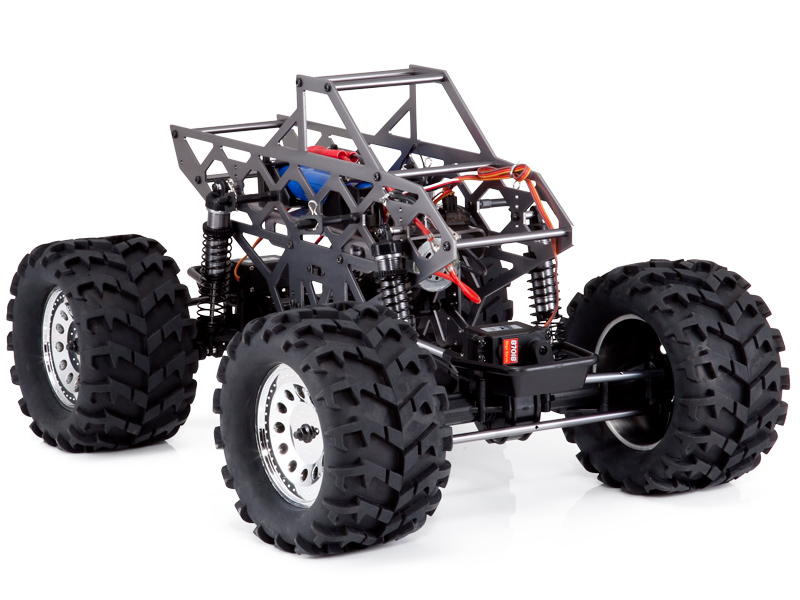
\includegraphics[width=10cm]{Chapters/Chapter2/Figures/groundpounder.jpg}
		\caption{Το τηλεκατευθυνόμενο όχημα \textit{GroundPounder}, της Redcat Racing.}
		\label{fig:groundpounder}
	\end{center}
\end{figure}

\bigskip
\subsection{Σασί Ρομποτικής Πλατφόρμας} \label{ssec:chassis}
Λόγω, της πληθώρας αισθητήρων, ηλεκτρονικού εξοπλισμού, καλωδιώσεων κλπ. και του περιορισμένου ελεύθερου χώρου πάνω στο όχημα, κρίθηκε σκόπιμο, αυτό, να επεκταθεί, με πρόσθετους χώρους. Για την λύση του προβλήματος, σχεδιάστηκαν, λοιπόν, και κατασκευάστηκαν, από μέλη της ομάδας P.A.N.D.O.R.A. 2014-15, δύο κουτιά, τα οποία προστέθηκαν επάνω στο υπάρχον όχημα, με σκοπό, να περιλάβουν τα επιμέρους υποσυστήματα του ρομπότ.

\begin{figure}[!ht]
	\centering
	\subfloat[Κουτί Τροφοδοσίας]{
		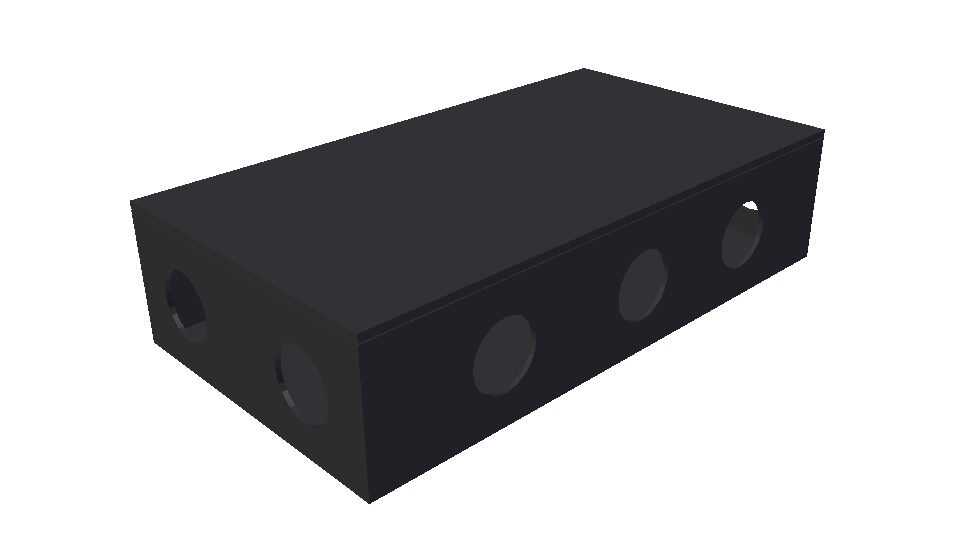
\includegraphics[width=0.45\linewidth]{Chapters/Chapter2/Figures/power_box.png}
		\label{fig:power_box}}
	\subfloat[Κουτί Ηλεκτρονικών]{
		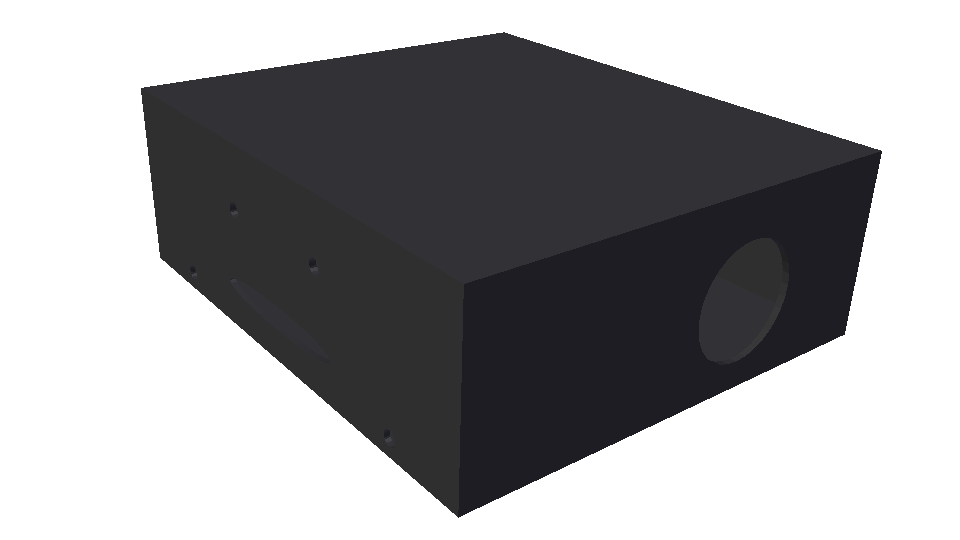
\includegraphics[width=0.45\linewidth]{Chapters/Chapter2/Figures/electronics_box.png}
		\label{fig:electronics_box}}
	\caption{Τα κουτιά του σασί της ρομποτικής πλατφόρμας Monstertruck.}
\end{figure}

\bigskip
Το \textit{κουτί τροφοδοσίας}, του σασί της ρομποτικής πλατφόρμας, που παρουσιάζεται στο σχήμα \ref{fig:power_box}, έχει διαστάσεις $310mm \times 170mm \times 74mm$, και περιλαμβάνει τρύπες, τοποθετημένες περιμετρικά του κουτιού, για πέρασμα καλωδιώσεων. Προορίζεται, όπως λέει και το όνομα του, για την τοποθέτηση του συστήματος τροφοδοσίας της ρομποτικής πλατφόρμας.

\bigskip
Το \textit{κουτί ηλεκτρονικών}, του σασί της ρομποτικής πλατφόρμας, που παρουσιάζεται στο σχήμα \ref{fig:electronics_box}, έχει διαστάσεις $210mm\times 240mm\times 84mm$, με δύο τρύπες στα πλάγια του ρομπότ, για τοποθέτηση ανεμιστήρων ψύξης του υπολογιστή, όπως, επίσης και ένα σύνολο από τρύπες στην μπροστινή πλευρά του κουτιού για κεραίες ασύρματης επικοινωνίας Wifi και καλωδιώσεις. Το \textit{κουτί ηλεκτρονικών}, προορίζεται για την τοποθέτηση του υπολογιστή, των αισθητήρων και των ελεγκτών της ρομποτικής πλατφόρμας.

\begin{figure}[!ht]
	\begin{center}
		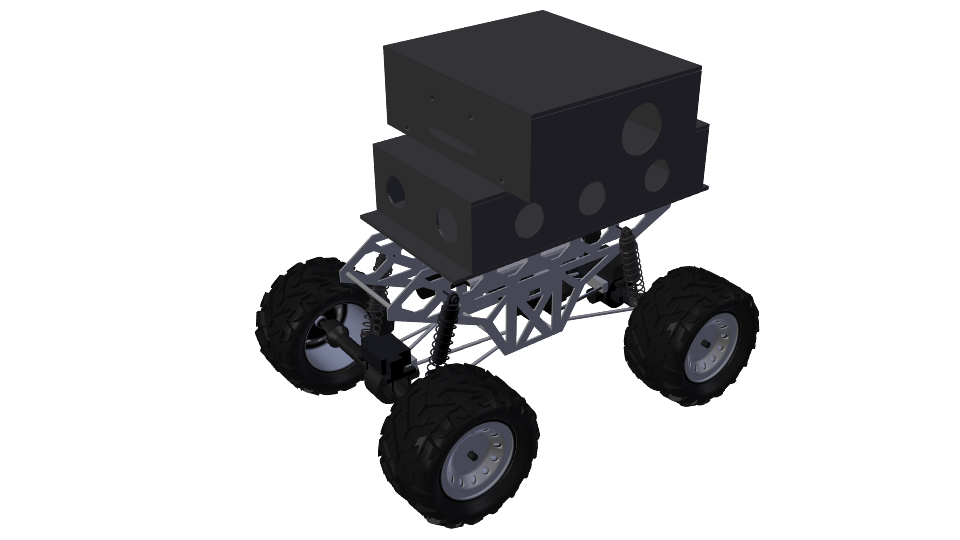
\includegraphics[width=10cm]{Chapters/Chapter2/Figures/base_diag.png}
		\caption{3D μοντέλο του συναρμολογημένου σασί της ρομποτικής πλατφόρμας Monstertruck.}
		\label{fig:chassis}
	\end{center}
\end{figure}

\bigskip
\subsection{Ηλεκτρονικός Εξοπλισμός} \label{ssec:electronic_equipment}
% σύστηματα τροφοδοσίας, υπολογιστής, αισθήτηρες, κινητήρες, σερβοκινητήρες και ελεγκτές

\bigskip
\subsubsection{Υπολογιστής} \label{sssec:computer}
Το πιο σημαντικό τμήμα ενός ρομποτικού συστήματος και ιδιαίτερα μίας αυτόνομης ρομποτικής πλατφόρμας αποτελεί ο εγκέφαλος του, δηλαδή, το υπολογιστικό του σύστημα, που του επιτρέπει να ελέγχει τα υποσυστήματα του και να εκτελεί διεργασίες και αλγορίθμους. Η επιλογή του υπολογιστικού συστήματος, που εν τέλει, εγκαταστάθηκε στην ρομποτική πλατφόρμα \textit{Monstertruck}, βασίστηκε σε δύο κριτήρια. Πρώτο και βασικότερο κριτήριο επιλογής, αποτέλεσε η υπολογιστική ισχύς και κατά πόσο θα μπορούσε να εκτελεί τους απαιτούμενους αλγορίθμους ταυτόχρονα, αποδοτικά και χωρίς καθυστερήσεις. Το δεύτερο κριτήριο επιλογής, που λήφθηκε υπόψιν, ήταν, η κατανάλωση ισχύος, όσον αφορά τον χρόνο αυτονομίας.

\bigskip
Με βάση τα παραπάνω κριτήρια, τα υπολογιστικά συστήματα που εξετάστηκαν είναι το \textit{Raspberry Pi 2}, του \textit{Raspberry Pi Foundation} και το \textit{Odroid-XU4}, της \textit{Hardkernel}. Και οι δύο υπολογιστές, αυτοί, αποτελούν πλήρεις υπολογιστές, με Κεντρική Μονάδα Επεξεργασίας (CPU), μνήμη RAM, κάρτα γραφικών κλπ., σε εξαιρετικά μικρό μέγεθος και χαμηλή κατανάλωση ισχύος.

\begin{figure}[!ht]
	\begin{minipage}[t]{.49\textwidth}
 		\centering
		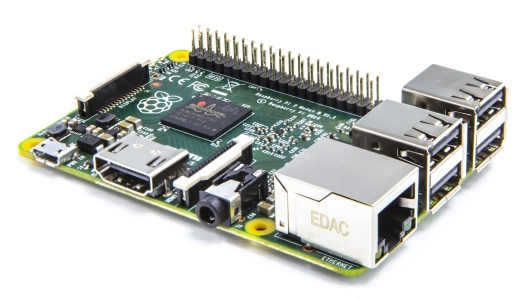
\includegraphics[width=0.6\linewidth]{Chapters/Chapter2/Figures/rpi2.jpg}
		\captionof{figure}{Raspberry Pi 2}
		\label{fig:rpi2}
	\end{minipage}
	\begin{minipage}[t]{.5\textwidth}		
		\centering
		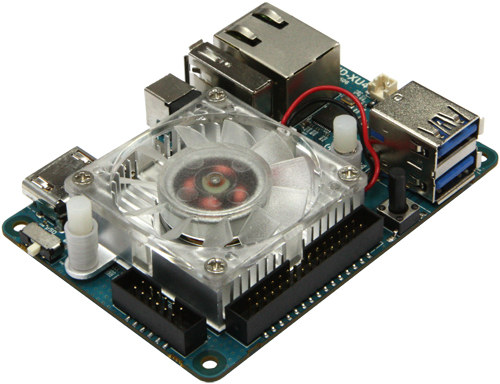
\includegraphics[width=0.5\linewidth]{Chapters/Chapter2/Figures/odroid-xu4.jpg}
		\captionof{figure}{Odroid-XU4}
		\label{fig:odroid-xu4}
	\end{minipage}
\end{figure}

\bigskip
\begin{table}[!ht]
	\centering
	\caption{Προδιαγραφές Raspberry Pi 2 και Odroid-XU4.}
	\begin{tabular}{| l | c | c |}
   		\hline
	   \textbf{Προδιαγραφές} & \textbf{Raspberry Pi 2} & \textbf{Odroid-XU4} \\ \hline
	   	CPU & Broadcom BCM2836 Arm7 & Samsung Exynos5422 ARM® \\ &Quad Core 900MHz Processor & Cortex™-A15 Quad 2.0GHz/\\ & & Cortex™-A7 Quad 1.4GHz\\ \hline
		GPU & Dual Core VideoCore IV® & Mali™-T628 MP6 OpenGL ES 3.0\\
		& Multimedia Co-Processor & / 2.0 / 1.1 and OpenCL 1.1 Full profile\\ 
		&  Open GL ES 2.0 &\\ \hline		   
	   Μνήμη RAM & 1GB LPDDR2 & 2GB LPDDR3 \\ \hline
	   Θύρες USB 2.0 & 4 & 1\\ \hline
	   Θύρες USB 3.0 & - & 2\\ \hline
	   Εικόνα & HDMI & HDMI\\ \hline
	   Ήχος & 4 pole Stereo output & HDMI Digital audio output\\ \hline
	   Αποθηκευτικός Χώρος & Micro SD & Micro SD ή eMMC 5.0\\ \hline
	   Ethernet & 10/100 & 10/100/1000\\ \hline
	  	Wifi & USB IEEE 802.11b/g/n & USB IEEE 802.11b/g/n 1T1R WLAN\\ \hline
	  	Περιφερειακά - & 40-pin GPIO, UART, SPI, I2C & UART, 30-pin GPIO/IRQ/SPI/ADC\\
	  	Διεπαφές & & 12-pin GPIO/I2S/I2C \\ \hline
	  	Τροφοδοσία & 5V, 2A & 5V, 4A\\ \hline
	   Διαστάσεις & $85 \times 56 \times 17 mm$ & $82 \times 58 \times 22 mm$\\\hline
   \end{tabular}
	\label{tab:computer_specs}
\end{table}

\newpage
Αρχικά, χρησιμοποιήθηκε, στην ρομποτική πλατφόρμα \textit{Monstertruck}, ο υπολογιστής \textit{Raspberry Pi 2}, αλλά, μετά από πειράματα και δοκιμές, με τους απαιτούμενους αλγορίθμους, για την αυτόνομη λειτουργία του οχήματος, διαπιστώθηκε, ότι, ο υπολογιστής \textit{Raspberry Pi 2},  είναι ανεπαρκής για την συγκεκριμένη εφαρμογή. Σαν αποτέλεσμα, στην ρομποτική πλατφόρμα, τελικά χρησιμοποιήθηκε ο υπολογιστής \textit{Odroid-XU4}, που μετά από αντίστοιχα πειράματα, η απόδοση του κρίθηκε πλήρως ικανοποιητική.

\bigskip
\subsubsection{Αισθητήρες} \label{sssec:sensors}
Μία εξαιρετικά σημαντική ιδιότητα, κάθε αυτόνομου ρομποτικού συστήματος, αποτελεί η αντίληψη του περιβάλλοντος του. Συγκεκριμένα, η ρομποτική αντίληψη στηρίζεται σε ένα σύνολο αισθητήρων, που επιτρέπουν στο ρομποτικό σύστημα να λαμβάνει πληροφορίες, σχετικά με το περιβάλλον του, σε μορφή κατανοητή και αξιοποιήσιμη από αυτό.

\bigskip
Οι ρομποτικοί αισθητήρες, χωρίζονται σε κατηγορίες, ανάλογα με την πηγή της πληροφορίας, σε \textit{ιδιοδεκτικούς (proprioceptive)} ή \textit{εξωδεκτικούς (exteroceptive)} \cite{autonomous_mobile_robots}, εάν η πληροφορία προέρχεται από το ίδιο το ρομποτικό σύστημα, ή από το περιβάλλον του, αντίστοιχα. Παραδείγματα \textit{ιδιοδεκτικών} αισθητήρων, αποτελούν, οι \textit{αισθητήρες μέτρησης θέσης, ταχύτητας και ροπής των κινητήρων}, \textit{γυροσκόπια}, \textit{αισθητήρες μέτρησης της φόρτισης των μπαταριών} κα. Αντίστοιχα, \textit{εξωδεκτικοί} αισθητήρες, θεωρούνται, οι \textit{αισθητήρες επαφής (tactile sensors)}, οι \textit{ηλεκτρονικές πυξίδες (compass, IMU)}, αισθητήρες \textit{GPS}, οι \textit{υπέρυθροι, υπερηχητικοί και λέιζερ αισθητήρες απόστασης (range sensors)}, όπως επίσης και οι \textit{κάμερες}. Επίσης, χωρίζονται και με βάση την πηγή εκπομπής της πληροφορίας \cite{autonomous_mobile_robots} σε \textit{παθητικούς (passive)}, εάν μετρούν κάποια μορφή ενέργειας που προέρχεται από το περιβάλλον και σε \textit{ενεργητικούς (active)}, εάν εκπέμπουν ενέργεια στο περιβάλλον και έπειτα, μετρούν την αντίδραση του περιβάλλοντος. Με βάση, τον συγκεκριμένο ορισμό, \textit{αισθητήρες αφής}, \textit{ηλεκτρονικές πυξίδες} και \textit{κάμερες}, αποτελούν \textit{παθητικούς} αισθητήρες, ενώ \textit{κωδικοποιητές(encoders) κινητήρων}, \textit{GPS}, \textit{αισθητήρες απόστασης}, αποτελούν \textit{ενεργητικούς} αισθητήρες. 

\bigskip
Ένα αυτόνομο ρομποτικό όχημα, είναι προφανές, ότι απαιτεί αισθητήρες, από όλες τις παραπάνω κατηγορίες για να μπορεί να αντιληφθεί και να κινηθεί μέσα στο περιβάλλον του, αλλά και να αντιδράσει μ' αυτό. Ακολούθως, παρουσιάζεται το σύνολο των αισθητήρων, που περιλαμβάνει η ρομποτική πλατφόρμα \textit{Monstertruck}.

\bigskip
\begin{enumerate}
% Laser Scanner
\item \textit{Σαρωτής Λέιζερ (Laser Scanner)}:\\
Οι πιο σημαντικοί αισθητήρες για ένα αυτόνομο ρομποτικό όχημα είναι οι \textit{αισθητήρες απόστασης (range sensors)}, οι οποίοι, του προσφέρουν πληροφορία, σχετικά με την απόσταση του οχήματος από εμπόδια, επιτρέποντας του, με αυτόν τον τρόπο, μέσω κατάλληλων αλγορίθμων, να χαρτογραφεί τον περιβάλλοντα χώρο του, να ξέρει, ανά πάσα στιγμή, τη θέση του και να πλοηγείται αυτόνομα μέσα σε αυτόν, αποφεύγοντας συγκρούσεις. 

Στην ρομποτική πλατφόρμα \textit{Monstertruck}, για τους παραπάνω λόγους, εγκαταστάθηκε ένας \textit{σαρωτής λέιζερ Hokuyo URG-04LX}. Η λειτουργία του βασίζεται στην τεχνική \textit{μέτρησης απόστασης, μέσω ανίχνευσης φωτός (Light Detection and Ranging - LIDAR)}. Δηλαδή, εκπέμπει έναν παλμό ακτινοβολίας λέιζερ στο περιβάλλον, προς μία κατεύθυνση και καταγράφοντας τον χρόνο που έκανε να επιστρέψει ο οπισθοσκεδαζόμενος παλμός, μπορεί να υπολογίσει την απόσταση του αισθητήρα από το περιβάλλον για εκείνη την κατεύθυνση. Πραγματοποιώντας την μέτρηση αυτή για ένα εύρος γωνιών, ο αισθητήρας προσφέρει μία διδιάστατη αναπαράσταση του περιβάλλοντος. 

\begin{figure}[!ht]
	\begin{minipage}[t]{.49\textwidth}
 		\centering
		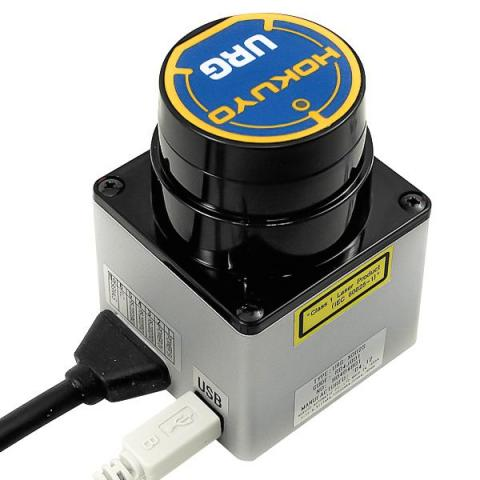
\includegraphics[width=0.6\linewidth]{Chapters/Chapter2/Figures/hokuyo.jpg}
		\captionof{figure}{Hokuyo URG-04LX.}
		\label{fig:hokuyo}
	\end{minipage}
	\begin{minipage}[t]{.49\textwidth}		
		\centering
 		\centering
		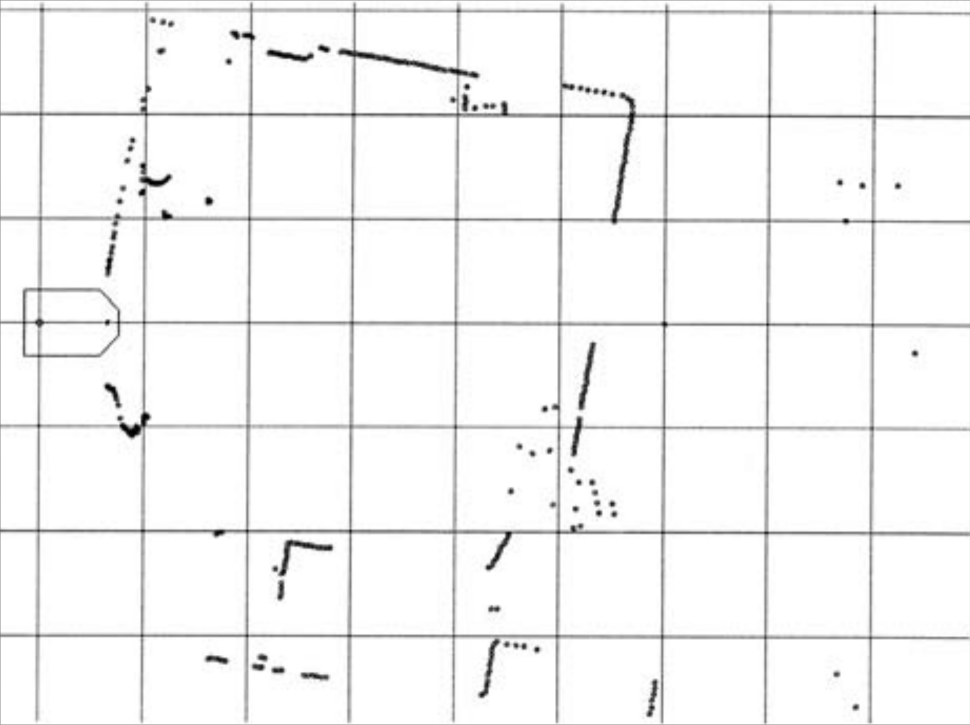
\includegraphics[width=0.75\linewidth]{Chapters/Chapter2/Figures/laser_scan.png}
		\captionof{figure}[Ενδεικτική σάρωση δωματίου.]{Ενδεικτική σάρωση δωματίου \cite{autonomous_land_vehicles}.}
		\label{fig:hokuyo_rays}
	\end{minipage}
\end{figure}

\bigskip

\begin{table}[!ht]
	\centering
	\captionof{table}{Προδιαγραφές Hokuyo URG-04LX}
	\label{tab:hokuyo_specs}
	\begin{tabular}{| l | c |}
		\hline
	   \textbf{Προδιαγραφές} & \textbf{Hokuyo URG-04LX} \\ \hline
	   Τροφοδοσία & 5VDC, 500mA\\ \hline
	   Εμβέλεια & 60 - 4\,095 mm \\ \hline
	   Περιοχή Μέτρησης & $240^{\circ}$\\ \hline
	   Ακρίβεια & $60 - 1000mm: \pm 10$ \\
   		& $1000 - 4095mm: 1\%$ \\ \hline
	  	Γωνιακή Ακρίβεια & $0.36^{\circ} (360^{\circ}/1024)$ \\ \hline
	  	Διεπαφή & USB, RS232 \\ \hline
	  	Διαστάσεις & $50 \times 50 \times 70 mm$ \\ \hline
	\end{tabular}
\end{table}

% IMU
\bigskip
\item \textit{Πυξίδα (Compass)}:\\
Ένα, άλλο είδος αισθητήρων, ιδιαίτερα δημοφιλές και απαραίτητο στις περισσότερες ρομποτικές εφαρμογές, αποτελούν οι \textit{αισθητήρες κατεύθυνσης (heading sensors)} \cite{autonomous_mobile_robots}. Στην κατηγορία, αυτή, ανήκουν τα \textit{γυροσκόπια (gyroscopes)}, τα \textit{κλινόμετρα (inclinometers)} και οι \textit{πυξίδες (compasses)}. Οι αισθητήρες, αυτοί, χρησιμοποιούνται για να καθοριστούν ο \textit{προσανατολισμός (orientation / yaw)} και η \textit{κλίση (pitch, roll)} του ρομποτικού οχήματος, αλλά και σε συνδυασμό με μετρήσεις ταχύτητας για την εκτίμηση της θέσης του (\textit{dead reckoning}).

Η ρομποτική πλατφόρμα \textit{Monstertruck} χρησιμοποιεί την \textit{πυξίδα Compass OS4000}, της \textit{Ocean Server}. Ο αισθητήρας αυτός, συνδυάζει ένα \textit{μαγνητόμετρο (magnetometer)}, τριών αξόνων και ένα \textit{επιταχυνσιόμετρο (accelerometer)}, τριών αξόνων. Το μαγνητόμετρο χρησιμοποιεί το μαγνητικό πεδίο της γης, για να μετρήσει τον απόλυτο προσανατολισμό, ως προς τους τρεις άξονες $x, y, z$, ενώ το επιταχυνσιόμετρο, μετράει μεταβολές στην ταχύτητα, ως προς τους τρεις άξονες $x, y, z$.

\begin{figure}[!ht]
	\begin{minipage}[b]{0.45\textwidth}
		\centering
		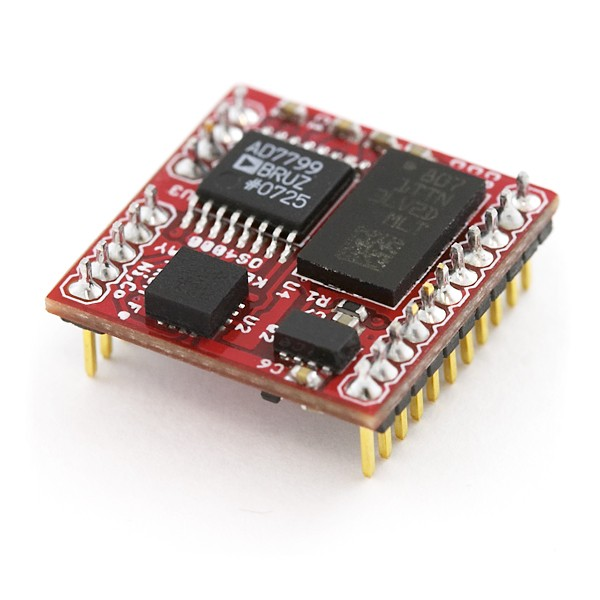
\includegraphics[width=0.5\linewidth]{Chapters/Chapter2/Figures/compassOS4000.jpg}
		\captionof{figure}{Compass OS4000.}
		\label{fig:compassOS4000}
	\end{minipage}		
	\begin{minipage}[b]{0.54\textwidth}
		\centering
		\captionof{table}{Προδιαγραφές Compass OS4000}
		\begin{tabular}{| l | c |}
			\hline
			\textbf{Προδιαγραφές} & \textbf{Compass OS4000}\\ \hline
			Τροφοδοσία & $3.3-5VDC, 30mA @ 3.3V$\\ \hline
			Σειριακή Διεπαφή& TTL 4800-115000 baud\\
			Επικοινωνίας  & 8 bit, 1 stop, no parity\\ \hline
			Συχνότητα & $0.01-40Hz$\\ \hline
			Ακρίβεια Αζιμούθιου & $<0.5^{\circ}, 0.1^{\circ}$ resolution\\ \hline
			Ακρίβεια Κλίσης & $<0.5^{\circ}, 0.1^{\circ}$ resolution\\ \hline
			Διαστάσεις & $15 \times 15 mm$\\ \hline
		\end{tabular}
		\label{tab:compassOS4000}
	\end{minipage}
\end{figure}

Η \textit{πυξίδα Compass OS4000}, χρησιμεύει, για την, εύρεση της κλίσης (pitch, roll) του ρομπότ, έτσι ώστε να σταθεροποιείται στο οριζόντιο επίπεδο ο \textit{σαρωτής λέιζερ}, που αναφέρθηκε παραπάνω, μέσω ενός μηχανισμού \textit{σταθεροποιητή pitch-roll}, που αποτελείται από δύο \textit{σερβοκινητήρες}. Παράλληλα, η \textit{πυξίδα} χρησιμοποιείται, και για στην εκτίμηση κατάστασης (θέση και προσανατολισμός) του οχήματος, συμπληρωματικά με άλλες πηγές εκτίμησης. Επίσης μπορεί να χρησιμοποιηθεί και για την επέκταση αλγορίθμων διάσχισης μονοπατιού, με βάση την ομαλότητα του εδάφους, βάση της τρέχουσα κλίσης του οχήματος, αλλά και σε ρουτίνες ασφαλείας, σε περίπτωση επικίνδυνων επιπέδων κλίσης του οχήματος, που μπορεί να προκαλέσουν ανατροπή.

% Camera
\bigskip
\item \textit{Κάμερα}:\\
Η όραση αποτελεί την πιο ισχυρή αίσθηση του ανθρώπου. Προσφέρει ένα τεράστιο όγκο πληροφορίας για το περιβάλλον και διευκολύνει την διάδραση του με αυτό. Στα ρομποτικά συστήματα, η αίσθηση της όρασης προσεγγίζεται με \textit{κάμερες}, οι οποίες καταγράφουν την ίδια πληροφορία, σε μεγάλο βαθμό που συγκεντρώνει και το ανθρώπινο μάτι.

Στα ρομποτικά συστήματα, \textit{κάμερες}, μπορεί να χρησιμοποιούνται για επίβλεψη και χειρισμό ρομποτικών συστημάτων, αλλά μεγαλύτερο ενδιαφέρον, παρουσιάζει ο κλάδος της \textit{ρομποτικής όρασης}, που ασχολείται με την δημιουργία αλγορίθμων, που εξάγουν πληροφορία, από τις εικόνες, που παράγει μία \textit{κάμερα}. Για παράδειγμα, \textit{κάμερες} και αλγόριθμοι \textit{ρομποτικής όρασης}, χρησιμοποιούνται για αναγνώριση αντικειμένων, προσώπων και προτύπων, γενικότερα, αλλά, ακόμα και σε \textit{χαρτογράφηση περιβάλλοντος} και \textit{εκτίμηση κατάστασης (Visual SLAM} κα.

Στην ρομποτική πλατφόρμα \textit{Monstertruck}, είναι εγκατεστημένη, μία απλή \textit{web κάμερα Logitech Portable Webcam C905}, η οποία, χρησιμοποιήθηκε, στα πλαίσια της παρούσας εργασίας, μονάχα για επίβλεψη κατά τον χειρισμό, ή την αυτόνομη λειτουργία της ρομποτικής πλατφόρμας. Παρόλα αυτά, όπως αναφέρθηκε παραπάνω, με την εκμετάλλευση της πληροφορίας από την κάμερα, μέσω κατάλληλων αλγορίθμων, η λειτουργικότητα της ρομποτικής πλατφόρμας, μπορεί να επεκταθεί σημαντικά.

\begin{figure}[!ht]
	\centering
	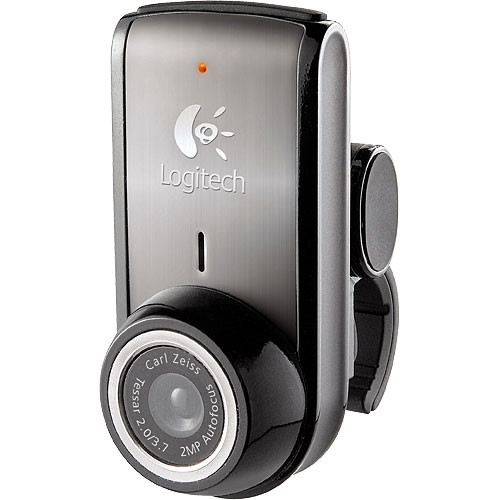
\includegraphics[width=.3\linewidth]{Chapters/Chapter2/Figures/webcam.jpg}
	\caption{Logitech Portable Webcam C905.}
	\label{fig:webcam}
\end{figure}


% motor encoders, hall sensors
\bigskip
\item \textit{Αισθητήρες Θέσης και Ταχύτητας Κινητήρων}:\\
Σε ρομποτικά συστήματα, με κινούμενα μέρη, όπως είναι προφανές, χρησιμοποιούνται κινητήρες και σερβοκινητήρες. Για τον ακριβή έλεγχο και παρακολούθηση, αυτών, είναι απαραίτητη η ύπαρξη αισθητήρων, που προσφέρουν πληροφορία, σχετικά με την θέση, ταχύτητα, επιτάχυνση, φορτίο, ρεύμα, τροφοδοσία ή θερμοκρασία, κατά την λειτουργία τους. Στη ρομποτική πλατφόρμα \textit{Monstertruck}, χρησιμοποιείται, ένας \textit{αισθητήρες Hall}, για τον κινητήρα των τροχών και \textit{κωδικοποιητές (encoders)}, για τον κινητήρα και τους σερβοκινητήρες του οχήματος. 

Ο \textit{αισθητήρας Hall}, είναι ένας μετατροπέας, που μεταβάλλει την τάση εξόδου του, ως αντίδραση στις μεταβολλές ενός μαγνητικού πεδίου. Στους κινητήρες χρησιμοποιείται ως μετρητής των στροφές ανά λεπτό. Είναι οικονομικός αισθητήρας, μπορεί να δουλέψει σε υψηλές συχνότητες και δεν επηρεάζεται από φαινόμενα θορύβου μηχανικών επαφών (contact bounce), αλλά, έχει μικρή ακρίβεια και είναι επιρρεπείς σε σφάλματα ολίσθησης (drift).

Οι \textit{κωδικοποιητές}, είναι μία κατηγορία αισθητήρων που χρησιμοποιούνται, για την μέτρηση της θέσης ή ταχύτητας του άξονα ενός κινητήρα. Η μέτρηση αυτή χρησιμοποιείται από το κύκλωμα κλειστού βρόχου, ενός κινητήρα για έλεγχο θέσης ή ταχύτητας. Οι απλοί, \textit{συμβατικοί σερβοκινητήρες (hobby servos)}, του εμπορίου, χρησιμοποιούν \textit{περιστροφικούς κωδικοποιητές} στην μορφή ποτενσιομέτρων (\textit{rotary / shaft encoders}), που μεταβάλλουν την τάση εξόδου τους, ανάλογα με την θέση του άξονα του σερβοκινητήρα. Αντίθετα, οι \textit{βιομηχανικοί κινητήρες}, συνήθως χρησιμοποιούν \textit{οπτικούς κωδικοποιητές (optical encoders)}, οι οποίοι, αποτελούνται από έναν δίσκο με διαφανείς και αδιαφανείς περιοχές και και ζεύγη φωτοεκπομπών και φωτοδεκτών, που διαβάζουν τα μοτίβα του δίσκου και συμπεραίνουν την θέση του άξονα του κινητήρα.

\begin{figure}[!ht]
	\centering
	\subfloat[Αισθητήρας Hall Κινητήρα.]{
		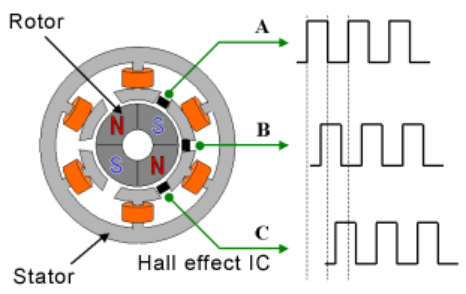
\includegraphics[width=0.3\linewidth]{Chapters/Chapter2/Figures/motor_hall_effect.png}
		\label{fig:hall_sensor}}
	\subfloat[Σερβοκινητήρας με περιστροφικό κωδικοποιητή.]{
		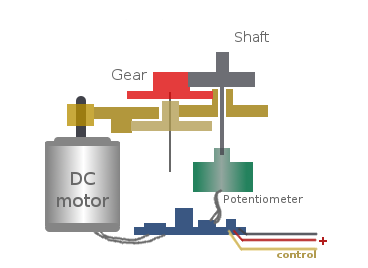
\includegraphics[width=0.35\linewidth]{Chapters/Chapter2/Figures/servo_internals.png}
		\label{fig:rotary_encoder}}\\
	\subfloat[Οπτικός κωδικοποιητής.]{
		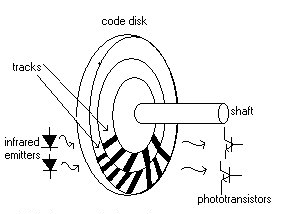
\includegraphics[width=0.3\linewidth]{Chapters/Chapter2/Figures/optical_encoder.png}
		\label{fig:optical_encoder}}
	\caption{Αισθητήρες θέσης και ταχύτητας κινητήρων.}
\end{figure}


% battery monitor
\bigskip
\item \textit{Αισθητήρας Μέτρησης Τάσης Μπαταρίας}:\\
Η ρομποτική πλατφόρμα \textit{Monstertruck}, τροφοδοτείται, μέσω, επαναφορτιζόμενων μπαταριών \textit{Λιθίου - Πολυμερών (LiPo)}, που συνδυάζουν υψηλή χωρητικότητα, μικρό όγκο και βάρος, σε σύγκριση με άλλους τύπους μπαταριών. Ένα σημαντικό πρόβλημα των μπαταριών \textit{LiPo}, είναι η ασφάλεια τους, καθώς σε περίπτωση υπερφόρτισης, αποφόρτισης, βραχυκυκλώματος, κρούσης ή διείσδυσης, μπορεί να προκληθεί καταστροφική ζημιά, όπως ρήξη συσκευασίας, διαρροή ηλεκτρολύτη και φωτιά. Επίσης, κακή χρήση της μπαταρίας, μέσω υπερφορτίσεων και αποφορτίσεων πέρα από τα επιτρεπτά επίπεδα, προκαλεί μείωση της χωρητικότητας και του χρόνου ζωής της μπαταρίας. Καθίσταται, επομένως, απαραίτητη, η χρήση ενός αισθητήρα, που θα μετρά τα επίπεδα τάσης της μπαταρίας και θα τα μεταδίδει στον κεντρικό υπολογιστή του ρομποτικού συστήματος, στον οποίο θα λειτουργεί μία διεργασία, που θα λαμβάνει την πληροφορία αυτή, θα την επεξεργάζεται κατάλληλα (πχ. φιλτράρισμα θορύβου) και θα εξάγει συμπεράσματα και θα ειδοποιεί τον επιβλέπον / χειριστή, σε περίπτωση που η μπαταρία χρειάζεται φόρτιση ή σε περίπτωση που παρεκκλίνει από τα επιτρεπτά όρια.

Για την μέτρηση της τάσης της μπαταρίας, απαιτείται ένας αισθητήρας που θα μετατρέπει την αναλογική τάση σε ψηφιακή πληροφορία. Τον σκοπό αυτό εξυπηρετούν οι \textit{Μετατροπείς Αναλογικού Σήματος σε Ψηφιακό (ADC)}, οι οποίοι μετατρέπουν μία αναλογική τάση σε έναν ψηφιακό αριθμό. Η διαδικασία της μετατροπής, περιλαμβάνει κβαντισμό και περιοδική δειγματοληψία, της τάσης εισόδου και σαν αποτέλεσμα εισάγει ένα μικρό σφάλμα μετατροπής, το οποίο στην προκειμένη περίπτωση, δεν επηρεάζει, σημαντικά, την εφαρμογή. Οι αισθητήρες \textit{ADC}, περιγράφονται, συνήθως, από μία μέγιστη τάση εισόδου (πχ. $5V$). Επειδή, όμως στην ρομποτική πλατφόρμα χρησιμοποιούνται μπαταρίες LiPo, με ονομαστική τάση $22.2V$ (μέγιστη τάση $25.2V$), απαιτείται μία κλιμάκωση της τάσης εισόδου. Για τον λόγο αυτό, η τάση εισόδου του μετατροπέα ADC, κλιμακώνεται, μέσω ενός διαιρέτη τάσης, με σχέση 1:10, από 0-25.2V σε 0-2.52V. Επίσης, λόγω των μεγάλων διαταραχών, στην τάση της μπαταρίας, κατά την λειτουργία της ρομποτικής πλατφόρμας, χρησιμοποιήθηκε ένα \textit{χαμηλοπερατό φίλτρο RC}. 

\begin{figure}[!ht]
	\centering
	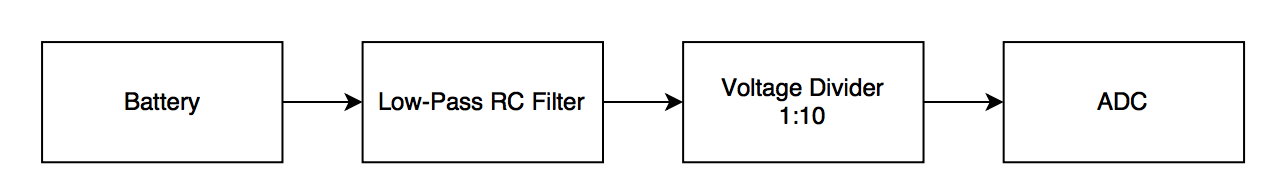
\includegraphics[width=\linewidth]{Chapters/Chapter2/Figures/rc_filter_divider.png}
	\caption{Στάδια επεξεργασίας τάσης μπαταρίας για μέτρηση της σε ADC.}
	\label{fig:rc_filter_divider}
\end{figure}

\end{enumerate}
%%%%%%%%%%%%%%%%%%%%%%%%%%%%%%%%%%%%%%%%%%%%%%%%%%%%%%%%%%%%%%%%%%%%%%%%%%%%%%%%%%%%%%%%%%%%%%

\bigskip
\subsubsection{Κινητήρας} \label{sssec:motor}
Το τηλεκατευθυνόμενο όχημα GroundPounder, αρχικά, περιελάμβανε έναν \textit{Brushed DC ηλεκτρικό κινητήρα}, με μέγιστη ταχύτητα, περίπου, $30\,000rpm$, ο οποίος ελεγχόταν από έναν ελεγκτή \textit{ESC}, με δυνατότητες ελέγχου ταχύτητας και φοράς. Παρόλα αυτά, λόγω της μικρής ακρίβειας, ελέγχου ταχύτητας και την απουσία \textit{κωδικοποιητή} ή άλλων αισθητήρων για την παροχή μετρήσεων, σχετικά την πραγματική ταχύτητα του κινητήρα, κάθε στιγμή, σε συνδυασμό, με τις υψηλές απαιτήσεις ακριβείας των ρομποτικών εφαρμογών, κρίθηκε σκόπιμο, το εν λόγω σύστημα κινητήρα και ελεγκτή, να αντικατασταθεί.

\begin{figure}[!ht]
	\begin{minipage}{.49\textwidth}
 	\centering
		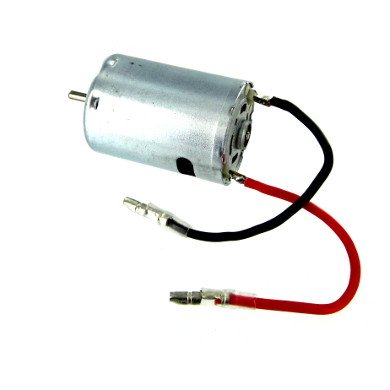
\includegraphics[width=0.6\linewidth]{Chapters/Chapter2/Figures/original_motor.jpg}
		\captionof{figure}{
			Ο κινητήρας Brushed 540 του τηλεκατευθυνόμενου οχήματος GroundPounder.}
		\label{fig:original_motor}
	\end{minipage}
	\begin{minipage}{.5\textwidth}		
		\centering
		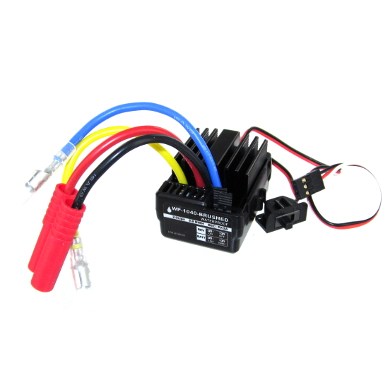
\includegraphics[width=0.6\linewidth]{Chapters/Chapter2/Figures/esc.jpg}
		\captionof{figure}{
			Ο ελεγκτής ESC B7003SR του τηλεκατευθυνόμενου οχήματος GroundPounder.}
		\label{fig:esc}
	\end{minipage}
\end{figure}

\bigskip
Για την αντικατάσταση, λοιπόν του παραπάνω συστήματος κινητήρα και ελεγκτή, επιλέχθηκαν, από τον διαθέσιμο εξοπλισμό της ομάδας \textit{P.A.N.D.O.R.A}, ένας κινητήρας, με αντίστοιχο ελεγκτή, της εταιρείας \textit{maxon motor}. Ο κινητήρας \textit{maxon EC-max 283858}, είναι ένας \textit{Brushless EC κινητήρας}, με μέγιστη ταχύτητα $18000rpm$, με \textit{ψηφιακό κωδικοποιητή (encoder)}, για μέτρηση της θέσης του άξονα του κινητήρα, όπως επίσης και \textit{αισθητήρα Hall} για μέτρηση των στροφών του κινητήρα, ανά λεπτό. Επίσης, περιλαμβάνει ένα \textit{κιβώτιο ταχυτήτων - μειωτήρα στροφών(gearbox) v842795-1-5}, με σχέση 1:66. 

\bigskip
Αντίστοιχα, ως ελεγκτής, επιλέχθηκε ο \textit{EPOS 24/1}, της \textit{maxon motor}. Ο ελεγκτής αυτός, αποτελεί ένα μικρού μεγέθους, ψηφιακό, έξυπνο ελεγκτή, με δυνατότητες ελέγχου 
θέσης, ταχύτητας και ρεύματος, αλλά και δυνατότητες μέτρησης θέσης και ταχύτητας του κινητήρα.

\begin{figure}[!ht]
	\begin{minipage}[b]{.49\textwidth}		
		\centering
		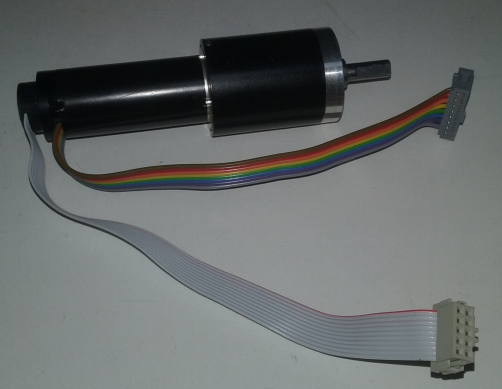
\includegraphics[width=0.8\linewidth]{Chapters/Chapter2/Figures/maxon_motor_ec_283858.png}
		\captionof{figure}{
			Ο κινητήρας maxon EC-max 283858, με κωδικοποιητή και μειωτήρα στροφών.}
		\label{fig:maxon_motor}
	\end{minipage}
	\begin{minipage}[b]{.5\textwidth}
 	\centering
		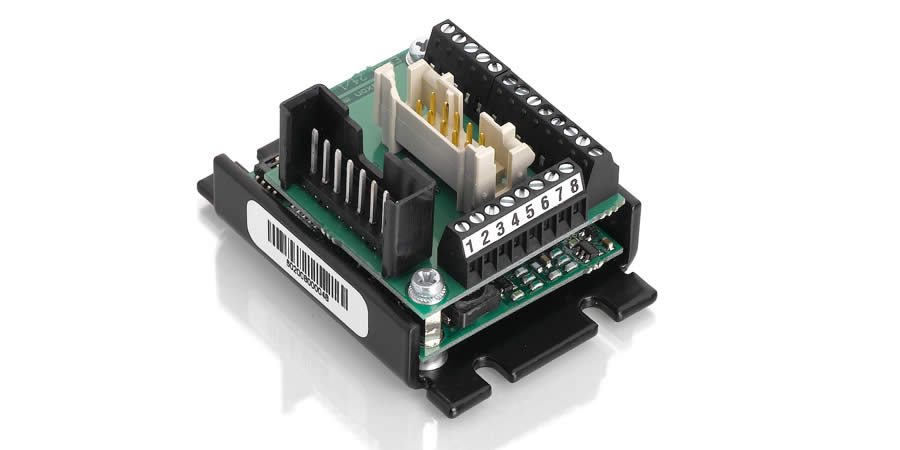
\includegraphics[width=0.8\linewidth]{Chapters/Chapter2/Figures/epos241.jpg}
		\captionof{figure}[Ο έξυπνος ελεγκτής κινητήρα, EPOS 24/1, της maxon motor.]{
			Ο έξυπνος ελεγκτής κινητήρα, EPOS 24/1, της maxon motor \cite{epos241_manual}.}	
		\label{fig:epos241}
	\end{minipage}
\end{figure}

Ο κινητήρας, συνδέεται με τον ελεγκτή \textit{EPOS 24/1}, μέσω δύο καλωδίων, ένα για τον έλεγχο του κινητήρα και για λήψη μετρήσεων από τον \textit{αισθητήρα Hall} και το άλλο, για λήψη μετρήσεων από τον \textit{ψηφιακό κωδικοποιητή}. Ο ελεγκτής \textit{EPOS 24/1}, επίσης, απαιτεί σύνδεση σε τροφοδοσία 9-24VDC, 1Α, ενώ παράλληλα, για επικονωνία με ηλεκτρονικό υπολογιστή, χρησιμοποιεί το πρωτόκολλο επικοινωνίας \textit{RS232}, χωρίς χειραψία, μέσω της ελάχιστης συνδεσμολογίας \textit{RS232} (RX, TX, Ground).

\begin{figure}[!ht]
		\centering
		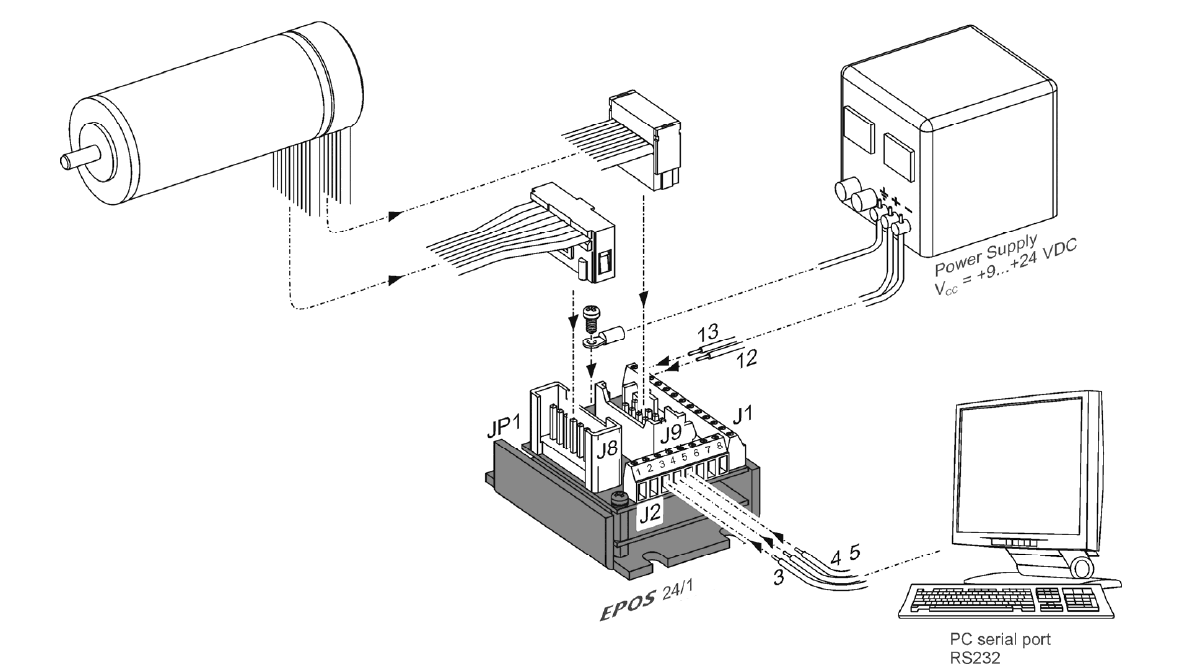
\includegraphics[width=0.7\linewidth]{Chapters/Chapter2/Figures/motor_minimum_wiring.png}
		\caption[Καλωδίωση Κινητήρα, Ελεγκτή και Υπολογιστή.]{Καλωδίωση Κινητήρα, Ελεγκτή και Υπολογιστή \cite{epos241_manual}.}
		\label{fig:motor_minimum_wiring}
\end{figure}

O ελεγκτής \textit{EPOS 24/1}, όπως προαναφέρθηκε, επιτρέπει την επικοινωνία με τον κεντρικό υπολογιστή της ρομποτικής πλατφόρμας, μέσω του πρωτοκόλλου διεπαφής \textit{RS232}. Παρόλα αυτά, ο κεντρικός υπολογιστής, δεν διαθέτει διεπαφή \textit{RS232} και επομένως, απαιτείται, ένας ενδιάμεσος κόμβος, ο οποίος θα καθιστά δυνατή την επικοινωνία μεταξύ τους. Το ρόλο αυτό, στην προκειμένη περίπτωση, εξυπηρετεί ένα \textit{μετατροπέας διεπαφής RS232 σε USB} (σχήμα \ref{fig:rs232_to_usb_adapter}).

\begin{figure}[!ht]
		\centering
		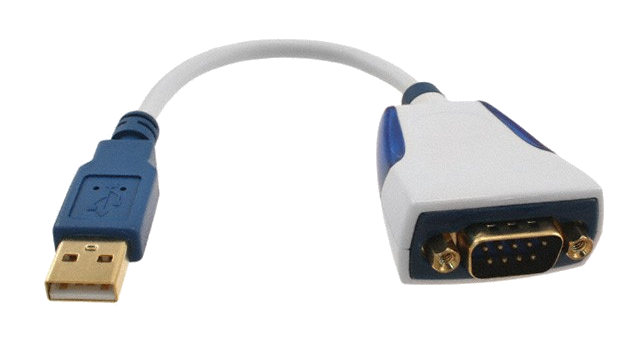
\includegraphics[width=.35\linewidth]{Chapters/Chapter2/Figures/rs232_to_usb_adapter.png}
		\caption{Μετατροπέας διεπαφής RS232 σε USB.}
		\label{fig:rs232_to_usb_adapter}
\end{figure}

\bigskip
\subsubsection{Σερβοκινητήρες} \label{sssec:servos}
Οι σερβοκινητήρες είναι κινητήρες, που επιτρέπουν ακριβή έλεγχο θέσης, ταχύτητας και επιτάχυνσης. Οι \textit{συμβατικοί σερβοκινητήρες} αποτελούνται από έναν DC κινητήρα, σε συνδυασμό με \textit{γρανάζια μετάδοσης}, έναν \textit{αισθητήρα θέσης}, συνήθως \textit{περιστροφικό κωδικοποιητή (rotary encoder)} και ένα κύκλωμα ελέγχου. Οι απλοί, συμβατικοί σερβοκινητήρες ελέγχονται, μέσω σημάτων Διαμόρφωσης Πλάτους Παλμού (PWM), αλλά υπάρχει, βέβαια και μία κατηγορία σερβοκινητήρων, οι λεγόμενοι \textit{έξυπνοι σερβοκινητήρες (smart servo motors)}, οι οποίοι έχουν ενσωματωμένο μικροελεγκτή. Ο μικροελεγτκής, αυτός, προσφέρει, υψηλότερη ακρίβεια ελέγχου, ευρωστία στο θόρυβο και αμφίδρομη επικοινωνία, μέσω σειριακού πρωτοκόλλου, συνήθως {TTL Full-Duplex} ή \textit{Half-Duplex} και \textit{RS485}. Τέλος, ένα σημαντικό πλεονέκτημα, των έξυπνων σερβοκινητήρων, έναντι των συμβατικών, είναι η παροχή μετρήσεων θέσης (position feedback), εξαιρετικής σημασίας για ρομποτικές εφαρμογές.

\bigskip
Στην ρομποτική πλατφόρμα \textit{Monstertruck} χρησιμοποιούνται συνολικά τέσσερις σερβοκινητήρες, δύο από τους οποίους είναι \textit{συμβατικοί} και οι άλλοι δύο, \textit{έξυπνοι}.

\bigskip
Οι δύο \textit{συμβατικοί σερβοκινητήρες}, χρησιμοποιούνται στο σύστημα \textit{τετραδιεύθυνσης} της ρομποτικής πλατφόρμας, που θα αναλυθεί στην αντίστοιχη ενότητα, είναι τύπου \textit{Hitek HS-M7990TH}, με ροπή $44 kg \cdot cm στα 6V$ και ανάλυση 0.082°/μsec.

\bigskip
Ο έλεγχος των δύο σερβοκινητήρων πραγματοποιείται από έναν ελεγκτή \textit{Micro Maestro 6 - Channel USB Servo Controller}, της \textit{Pololu}. Ο ελεγκτής, αυτός, προσφέρει αποδοτικό έλεγχο σερβοκινητήρων, υψηλής ακρίβειας, με ενσωματωμένο έλεγχο ταχύτητας και επιτάχυνσης, έξι κανάλια ελέγχου και επικοινωνία, μέσω σειριακού πρωτοκόλλου \textit{USB}.

\begin{figure}[!ht]
	\begin{minipage}[t]{.49\textwidth}		
		\centering
		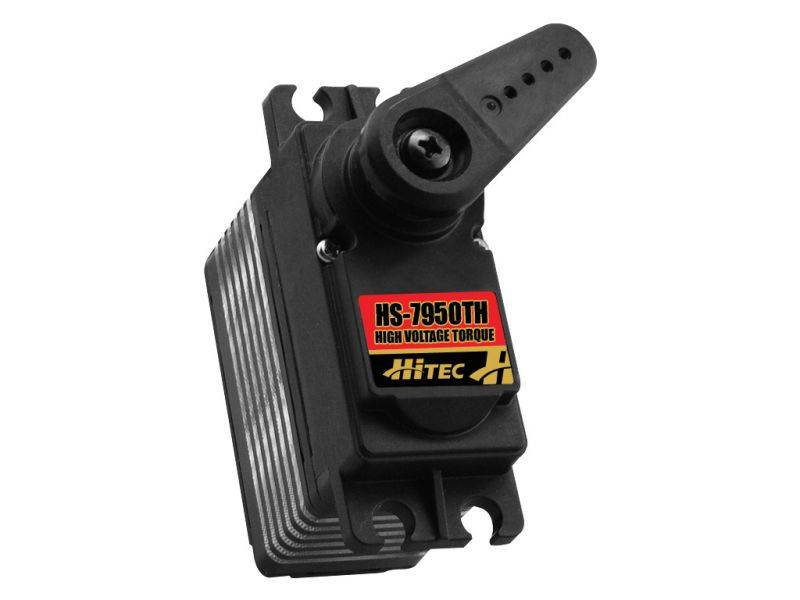
\includegraphics[width=0.5\linewidth]{Chapters/Chapter2/Figures/hitek_servo.jpg}
		\caption{Σερβοκινητήρας Hitek HS-7954TH.}
		\label{fig:hitek_servo}
	\end{minipage}
	\begin{minipage}[t]{.5\textwidth}
 	\centering
		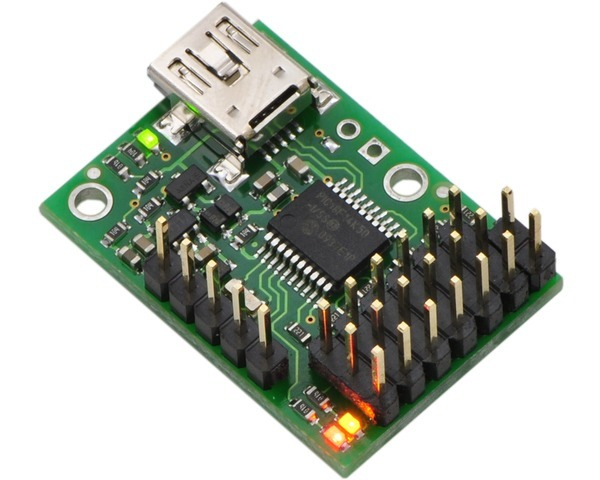
\includegraphics[width=0.5\linewidth]{Chapters/Chapter2/Figures/pololu_maestro.jpg}
		\captionof{figure}{Pololu Micro Maestro 6-Channel USB Servo Controller}
		\label{fig:pololu_maestro}
	\end{minipage}
\end{figure}

\begin{figure}[!ht]
		\centering
		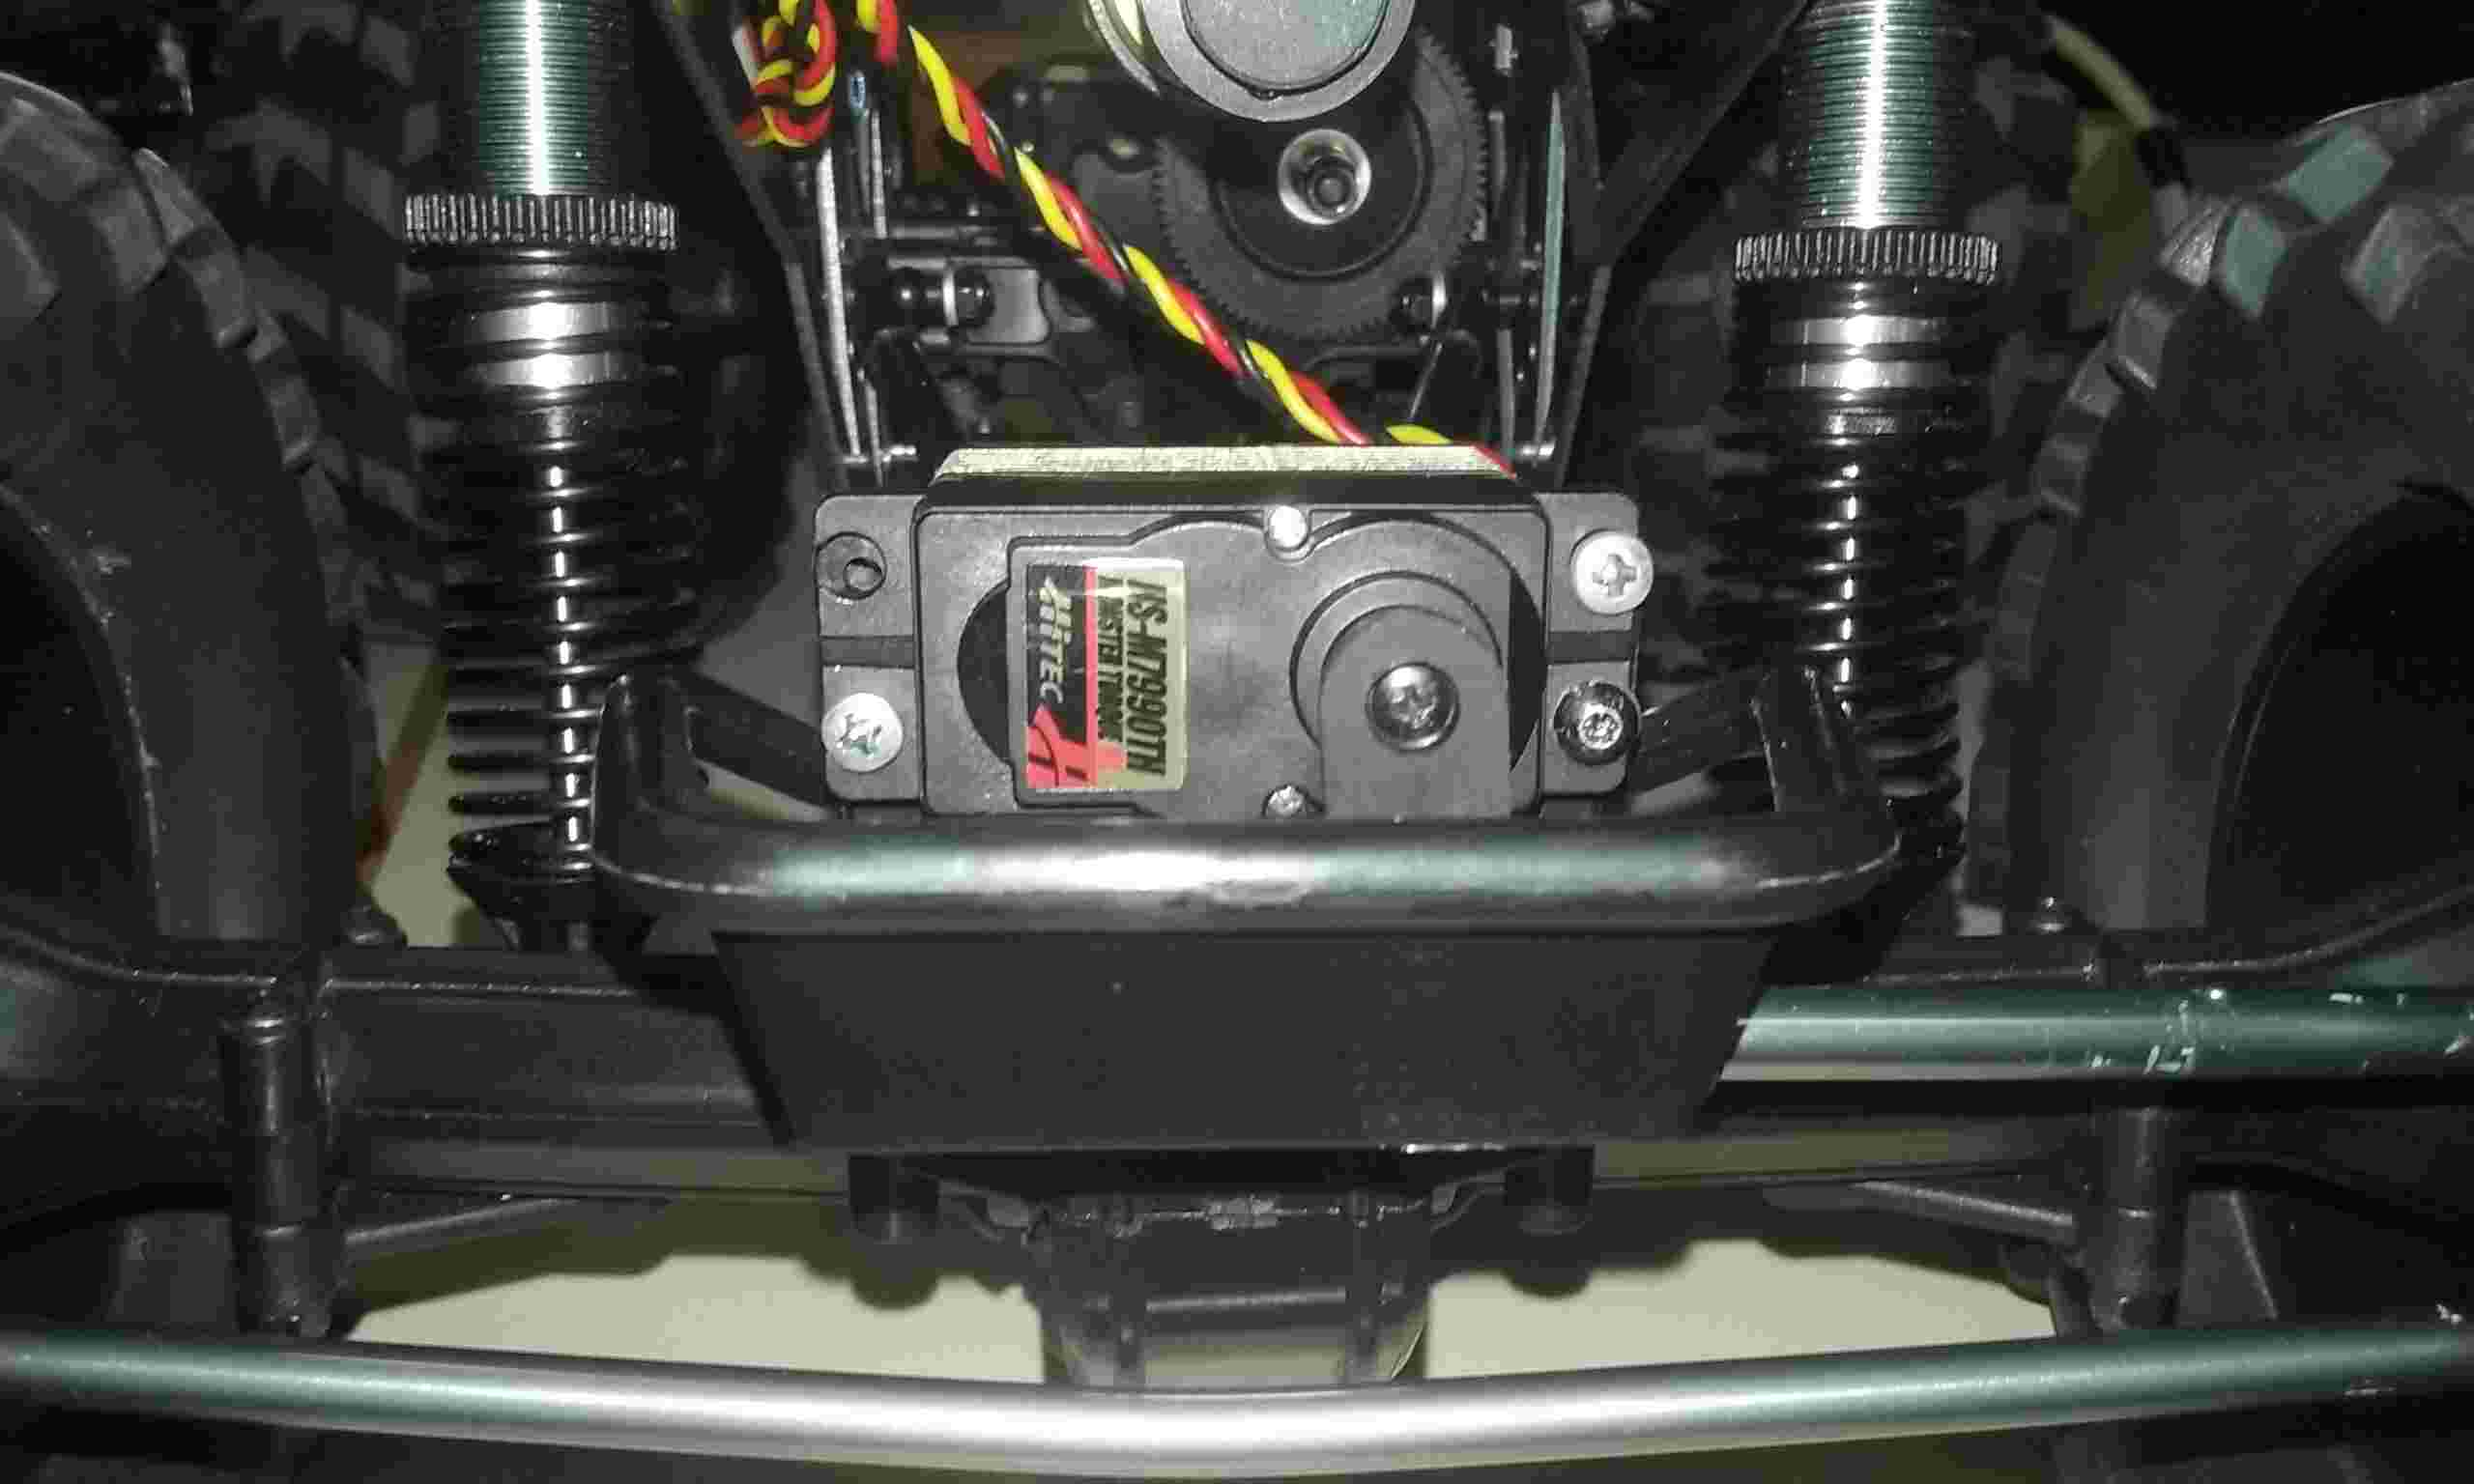
\includegraphics[width=0.5\linewidth]{Chapters/Chapter2/Figures/steering_servo.jpg}
		\caption{O Σερβοκινητήρας Hitek HS-7954TH πάνω στην ρομποτική πλατφόρμα Monstertruck.}
		\label{fig:servo_steering}
\end{figure}

\bigskip
Οι δύο \textit{έξυπνοι σερβοκινητήρες}, χρησιμοποιούνται ως \textit{μηχανισμός σταθεροποίησης (Pitch-Roll Stabilizer)} του \textit{Σαρωτή Λέιζερ}, που αναφέρθηκε παραπάνω, λαμβάνοντας υπόψιν πληροφορία για την κλίση του οχήματος, μέσω της πυξίδας \textit{Compass OS4000}. Ο μηχανισμός αυτός είναι απαραίτητος για την αξιόπιστη χαρτογράφηση χώρου με ανώμαλο έδαφος.

\bigskip
Οι \textit{έξυπνοι σερβοκινητήρες} του \textit{μηχανισμού σταθεροποίησης} του \textit{Σαρωτή Λέιζερ}, είναι τύπου \textit{Dynamixel AX-12A}, της \textit{Robotis}. Οι \textit{έξυπνοι σερβοκινητήρες Dynamixel AX-12}, έχουν την δυνατότητα, να παίρνουν μετρήσεις, σχετικά με την ταχύτητα, θέση, θερμοκρασία, τάση και φορτίο και να αντιδρούν ανάλογα με την περίπτωση και να μεταδίδουν αυτήν την πληροφορία, στον υπολογιστή του ρομποτικού συστήματος.

\begin{figure}[!ht]
	\begin{minipage}[b]{0.45\textwidth}
		\centering
		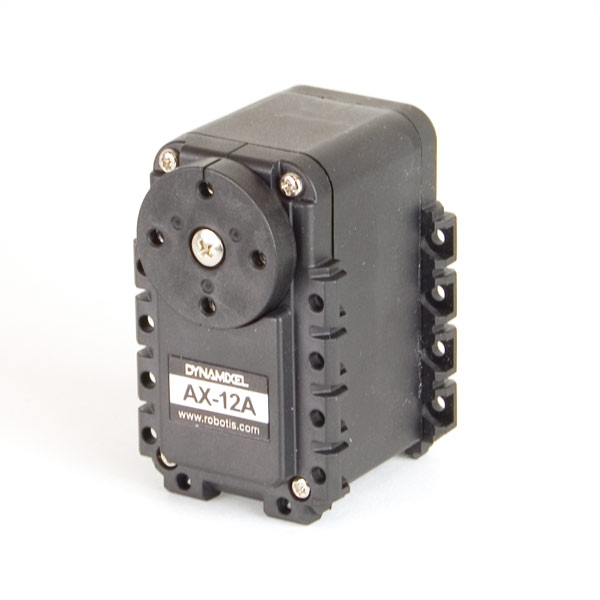
\includegraphics[width=0.8\linewidth]{Chapters/Chapter2/Figures/dxl_ax_12a.png}
		\caption{Σερβοκινητήρας Dynamixel\\ AX-12A, της Robotis.}
		\label{fig:dxl_ax_12a}
	\end{minipage}		
	\begin{minipage}[b]{0.475\textwidth}
		\centering
		\captionof{table}{Προδιαγραφές σερβοκινητήρα\\ Dynamixel AX-12A, της Robotis}
		\begin{tabular}{| l | c |}
			\hline
			\textbf{Προδιαγραφές} & \textbf{Dynamixel AX-12A}\\ \hline
			Τροφοδοσία & $9-12VDC, 900mA$\\ \hline
			Σειριακή Διεπαφή& 3-pin TTL Half-Duplex\\
			Επικοινωνίας  & 7343bps ~ 1Mbps\\ \hline
			Εύρος & $300^{\circ}$\\ \hline
			Μέγιστη Ροπή & $15.3 kg \cdot cm$\\ \hline
			Μέγιστη Ταχύτητα & 59 RPM \\ (χωρίς φορτίο) & 0.169sec/60°\\ \hline
			Feedback & Θέσης, Φορτίου,\\& Θερμοκρασίας, Τάσης\\ \hline
			Διαστάσεις & $32 \times 50 \times 40 mm$\\ \hline
		\end{tabular}
		\label{tab:dxl_ax_12a_specs}
	\end{minipage}
\end{figure}


\bigskip
Η επικοινωνία, μεταξύ του υπολογιστή και των \textit{έξυπνων σερβοκινητήρων}, επιτυγχάνεται μέσω του \textit{αντάπτορα USB2Dynamixel}, ο οποίος επικοινωνεί με τον υπολογιστή, μέσω σειριακού πρωτοκόλλου \textit{USB} και με τους \textit{έξυπνους σερβοκινητήρες}, μέσω σειριακής επιικοινωνίας \textit{TTL}. Επίσης, οι δύο \textit{έξυπνοι σερβοκινητήρες}, συνδέονται, μεταξύ τους, σειριακά, μέσω τοπολογίας \textit{Daisy Chain}.

\begin{figure}[!ht]
	\begin{minipage}[t]{.49\textwidth}
 	\centering
		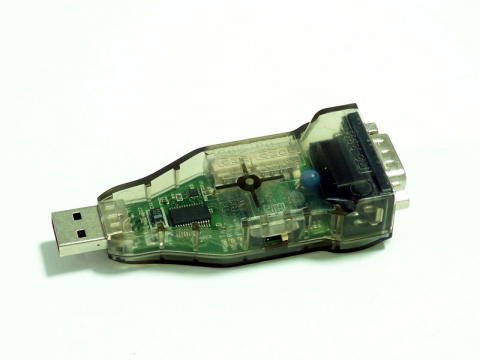
\includegraphics[width=0.6\linewidth]{Chapters/Chapter2/Figures/usb2dynamixel.png}
		\captionof{figure}{Αντάπτορας USB2Dynamixel,\\ της Robotis.}
		\label{fig:usb2dynamixel}
	\end{minipage}
	\begin{minipage}[t]{.5\textwidth}		
		\centering
		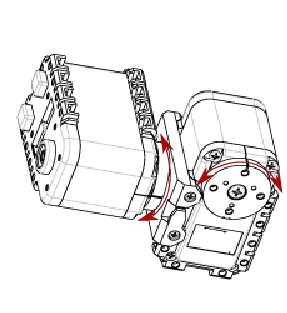
\includegraphics[width=0.5\linewidth]{Chapters/Chapter2/Figures/pitch_roll_dxl.png}
		\caption{Διάταξη Pitch-Roll του\\ σταθεροποιητή του σαρωτή λέιζερ.}
		\label{fig:pitch_roll_dxl}
	\end{minipage}
\end{figure}

\bigskip
\subsubsection{Ασύρματη Επικοινωνία} \label{sssec:wireless_communication}
Η προετοιμασία και ο χειρισμός της ρομποτικής πλατφόρμας \textit{Monstertruck}, ή η επίβλεψη της, κατά την αυτόνομη λειτουργία, από τον χειριστή/επιβλέποντα, απαιτεί έναν πρόσθετο υπολογιστή, ο οποίος θα συνιστά τον \textit{σταθμό χειρισμού/επίβλεψης}. Η επικοινωνία, μεταξύ των δύο υπολογιστικών συστημάτων, μπορεί να πραγματοποιηθεί, είτε ενσύρματα, μέσω μίας διασύνδεσης διεπαφής \textit{Ethernet}, είτε ασύρματα, μέσω ενός πομποδέκτη ασύρματης επικοινωνίας \textit{Wi-Fi}, σε συνδυασμό με έναν \textit{δρομολογητή Wi-Fi (Wi-Fi router)} που αποτελεί και την πιο πρακτική λύση, αν αναλογιστεί κανείς, ότι σε αντίθετη περίπτωση, ο χειριστής, θα έπρεπε να κυνηγάει το ρομπότ από πίσω, με κίνδυνο, πρόκλησης ατυχήματος, πιθανή αποσύνδεση, αλλά και πιθανή παρεμβολή στις μετρήσεις των αισθητήρων. H απαίτηση, αυτή, ικανοποιείται, στη ρομποτική πλατφόρμα \textit{Monstertruck}, μέσω ενός αντάπτορα \textit{TP-Link WiFi N900 TL-WDN4200}.

\bigskip
\begin{figure}[!ht]
	\begin{minipage}[b]{0.4\textwidth}
		\centering
		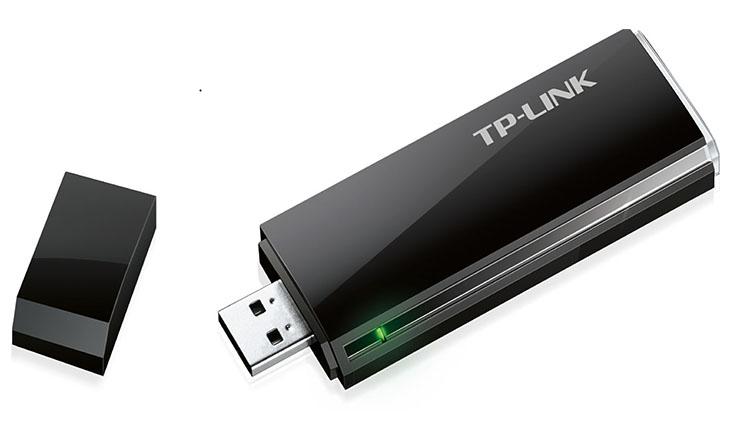
\includegraphics[width=0.6\linewidth]{Chapters/Chapter2/Figures/wifi_adapter.png}
		\caption{TP-Link Wi-Fi USB\\ Adapter N900 TL-WDN4200.}
		\label{fig:wifi_adapter}
	\end{minipage}		
	\begin{minipage}[b]{0.5\textwidth}
		\centering
		\captionof{table}{Προδιαγραφές TP-Link Wi-Fi USB\\ Adapter N900 TL-WDN4200.}
		\begin{tabular}{| l | c |}
			\hline
			\textbf{Προδιαγραφές} & \textbf{TP-Link Wi-Fi USB Adapter}\\
			 &  \textbf{N900 TL-WDN4200}\\ \hline
			Σύνδεση & USB 2.0 \\ \hline
			Ταχύτητα & Dual Band $2 \times 450Mbps$\\ \hline
			Πρότυπο & IEEE 802.11b/g/n\\ \hline
			Συχνότητα & 2.4/5GHz\\ \hline
			Ασφάλεια & WEP (64-128bit)\\ \hline
		\end{tabular}
		\label{tab:wifi_adapter_specs}
	\end{minipage}
\end{figure}


\bigskip
\subsubsection{Διασύνδεση Υποσυστημάτων} \label{sssec:interconnections}
Στις παραπάνω ενότητες, αναφέρθηκαν τα επιμέρους υποσυστήματα της ρομποτικής πλατφόρμας \textit{Monstertruck} και έγινε φανερό, ότι δεν χρησιμοποιούνται οι ίδιες διεπαφές επικοινωνίας σε κάθε συσκευή, αλλά και ότι κάθε συσκευή, χρησιμοποιεί το δικό της πρωτόκολλο επικοινωνίας. Το μόνο κοινό όλων των υποσυστημάτων, είναι η διασύνδεση και η συγκέντρωση της πληροφορίας, στον κεντρικό κόμβο του συστήματος, τον υπολογιστή \textit{Odroid-XU4}.

\bigskip
Ένα σημαντικό πρόβλημα, του υπολογιστή \textit{Odroid-XU4}, αποτελεί ο ανεπαρκής, για την συγκεκριμένη εφαρμογή, αριθμός θυρών διεπαφής σειριακής επικοινωνίας USB. Επομένως, για την ταυτόχρονη λειτουργία, όλων των επιμέρους αισθητήρων και ελεγκτών του συστήματος, κρίθηκε απαραίτητη η προσθήκη δύο \textit{διακλαδωτών USB (USB Hubs)}(σχήμα \ref{fig:usb_hubs}X). Η διασύνδεση των διεπαφών, όλων των επιμέρους επιμέρους υποσυστημάτων, της ρομποτικής πλατφόρμας \textit{Monstertruck}, παρουσιάζεται στο σχήμα \ref{fig:hardware_interface_diagram}.

\begin{figure}[!ht]
	\centering
	\subfloat[Akasa AK-HB-01-BK 4-port USB hub Black.]{
		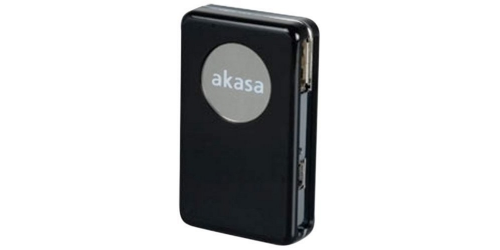
\includegraphics[width=0.33\linewidth]{Chapters/Chapter2/Figures/usb_hub_black.png}
		\label{fig:usb_hub_black}}
	\subfloat[Akasa AK-HB-01WH C 4-PORT USB hub White.]{
		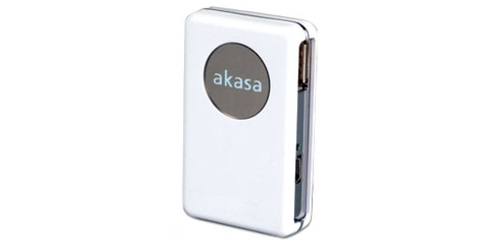
\includegraphics[width=0.33\linewidth]{Chapters/Chapter2/Figures/usb_hub_white.png}
		\label{fig:usb_hub_white}}
	\caption{Οι διακλαδωτές σειριακής διεπαφής USB (USB Hubs) της ρομποτικής  πλατφόρμας Monstertruck.}
	\label{fig:usb_hubs}
\end{figure}


\begin{figure}[!ht]
	\centering
	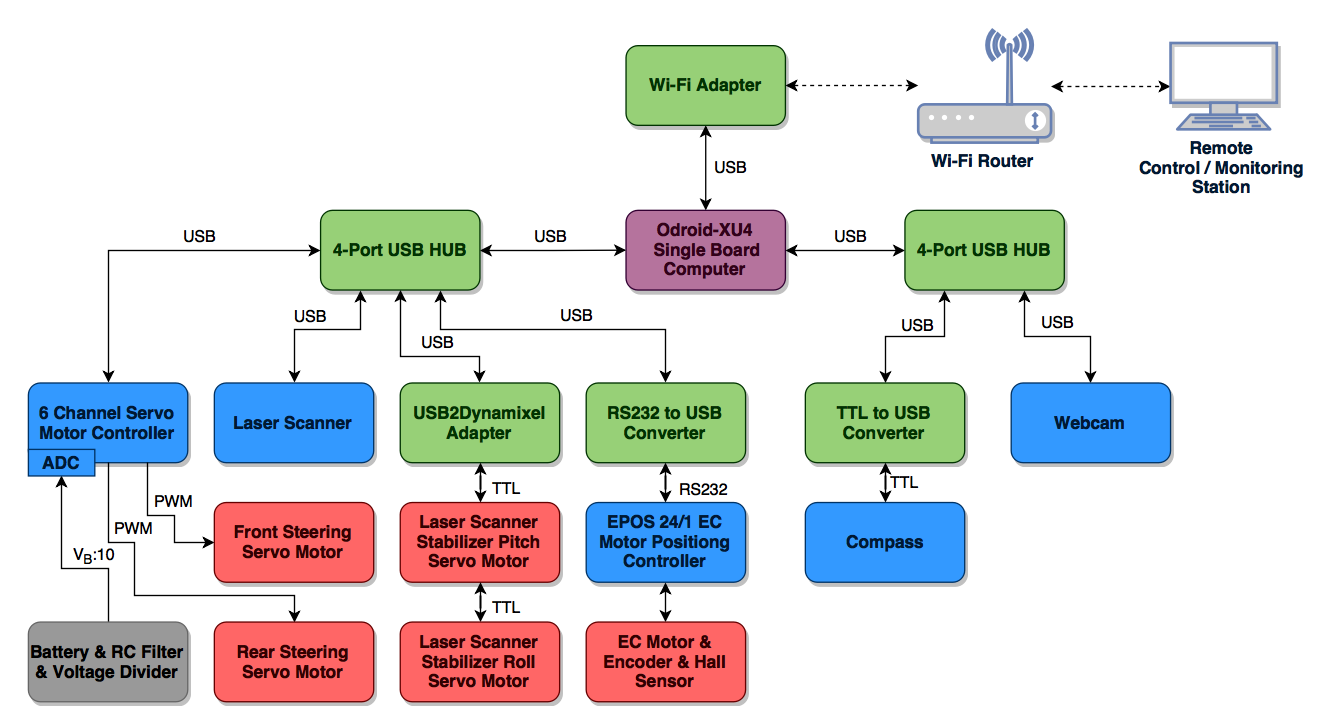
\includegraphics[width=1\linewidth]{Chapters/Chapter2/Figures/hardware_interface_diagram.png}
	\caption{Διασύνδεση διεπαφών των επιμέρους υποσυστημάτων της ρομποτικής πλατφόρμας \textit{Monstertruck}.}
	\label{fig:hardware_interface_diagram}
\end{figure}


\bigskip
\subsubsection{Σύστημα Τροφοδοσίας} \label{sssec:power_supply}
Από την παρουσίαση των επιμέρους υποσυστημάτων της ρομποτικής πλατφόρμας \textit{Monstertruck}, που πραγματοποιήθηκε στις προηγούμενες παραγράφους, προκύπτει, ότι, κάθε υποσύστημα - συσκευή, περιλαμβάνει διαφορετικές προδιαγραφές τροφοδοσίας. Επομένως, απαιτείται, ένα εκτενές και πλήρες σύστημα τροφοδοσίας, που να προσφέρει τις απαιτούμενες προδιαγραφές για κάθε υποσύστημα ξεχωριστά, για την ταυτόχρονη λειτουργία, όλων μαζί, αλλά και να επιτρέπει περιθώρια επέκτασης. Επίσης, θα πρέπει να περιλαμβάνει, επαρκής απομόνωση της τροφοδοσίας των ευαίσθητων ηλεκτρονικών υποσυστημάτων, από άλλα υποσυστήματα που εισάγουν θόρυβο στις γραμμές τροφοδοσίας, όπως οι κινητήρες και οι σερβοκινητήρες. 

\bigskip
Όπως, παρουσιάζεται και στο σχήμα \ref{fig:power_distribution}, ως πηγή τροφοδοσίας της ρομποτικής πλατφόρμας \textit{Monstertruck}, χρησιμοποιείται μία μπαταρία \textit{Λιθίου-Πολυμερών} (σχήμα \ref{fig:battery}) με ονομαστική τάση 22.2V, μέγιστη τάση 25.2V ($100\%$ φόρτιση) και 3700/4000/5000mAh. Η τροφοδοσία που παρέχει η μπαταρία, τροφοδοτείται σε έναν \textit{διακλαδωτή (Battery Distribution Board)}, από τον οποίο τροφοδοτούνται ο ελεγκτής \textit{EPOS 24/1} που τροφοδοτεί και τον κινητήρα του οχήματος, ο \textit{12V DC-DC μετατροπέας} και το \textit{τροφοδοτικό M4-ATX}.

\begin{figure}[!ht]
	\centering
	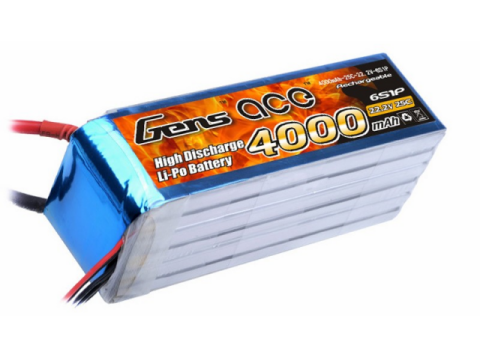
\includegraphics[width=0.25\linewidth]{Chapters/Chapter2/Figures/battery.png}
	\caption{Μπαταρία Gens ace, LiPo, 22.2V, 4000mAh.}
	\label{fig:battery}
\end{figure}

\bigskip
Ο \textit{12V DC-DC μετατροπέας} τροφοδοτεί με 12V, μέσω ενός \textit{διακλαδωτή (Motor Distribution Board)} τους \textit{έξυπνους σερβοκινητήρες Dynamixel}, του \textit{σταθεροποιητή Pitch-Roll} του \textit{σαρωτή λέιζερ}, όπως επίσης και έναν ανεμιστήρα, υπεύθυνο, για την ψύξη του υπολογιστή \textit{Odroid-XU4}.

\bigskip
Το τροφοδοτικό \textit{M4-ATX}, παράγει εξόδους τροφοδοσίας 5V και 12V και τροφοδοτεί την πλειονότητα των ηλεκτρονικών υποσυστημάτων της ρομποτικής πλατφόρμας. Αρχικά, τροφοδοτεί απευθείας έναν \textit{5V DC-DC μετατροπέα}, ο οποίος χρησιμοποιείται για να τροφοδοτεί τους σερβοκινητήρες του συστήματος στρέψης - \textit{τετραδιεύθυνσης} της ρομποτικής πλατφόρμας, απομονώνοντας, ταυτόχρονα την τροφοδοσία των σερβοκινητήρων από την τροφοδοσία των υπόλοιπων ηλεκτρονικών υποσυστημάτων, που παρουσιάζουν ευαισθησία στον θόρυβο. Τα υπόλοιπα ηλεκτρονικά υποσυστήματα της ρομποτικής πλατφόρμας, τροφοδοτούνται, από το τροφοδοτικό \textit{M4-ATX}, μέσω ενός \textit{διακλαδωτή (Electronics Distribution Board)}, είτε άμεσα, όπως ο υπολογιστής \textit{Odroid-XU4}, ο \textit{σαρωτής λέιζερ} και οι \textit{διακλαδωτές USB (USB Hubs)}, είτε μέσω του υπολογιστή και των \textit{διακλαδωτών USB}.

\begin{figure}[!ht]
	\centering
	\subfloat[Τροφοτικό M4-ATX.]{
		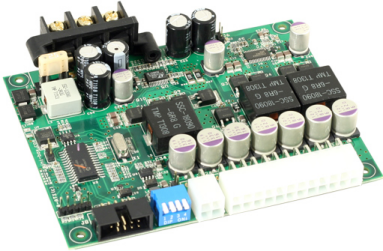
\includegraphics[width=0.3\linewidth]{Chapters/Chapter2/Figures/m4atx.png}
		\label{fig:m4atx}}
	\subfloat[5V DC-DC Μετατροπέας.]{
		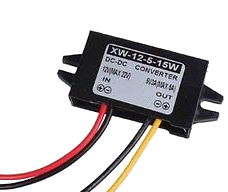
\includegraphics[width=0.3\linewidth]{Chapters/Chapter2/Figures/5v_dc_dc_converter.png}
		\label{fig:5v_dc_dc_converter}}
	\subfloat[12V DC-DC Μετατροπέας.]{
		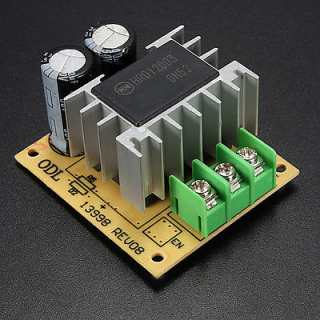
\includegraphics[width=0.3\linewidth]{Chapters/Chapter2/Figures/12v_dc_dc_converter.png}
		\label{fig:12v_dc_dc_converter}}
	\caption{Επιμέρους τμήματα συστήματος τροφοδοσίας.}
\end{figure}

\bigskip
\begin{figure}[!ht]
	\centering
	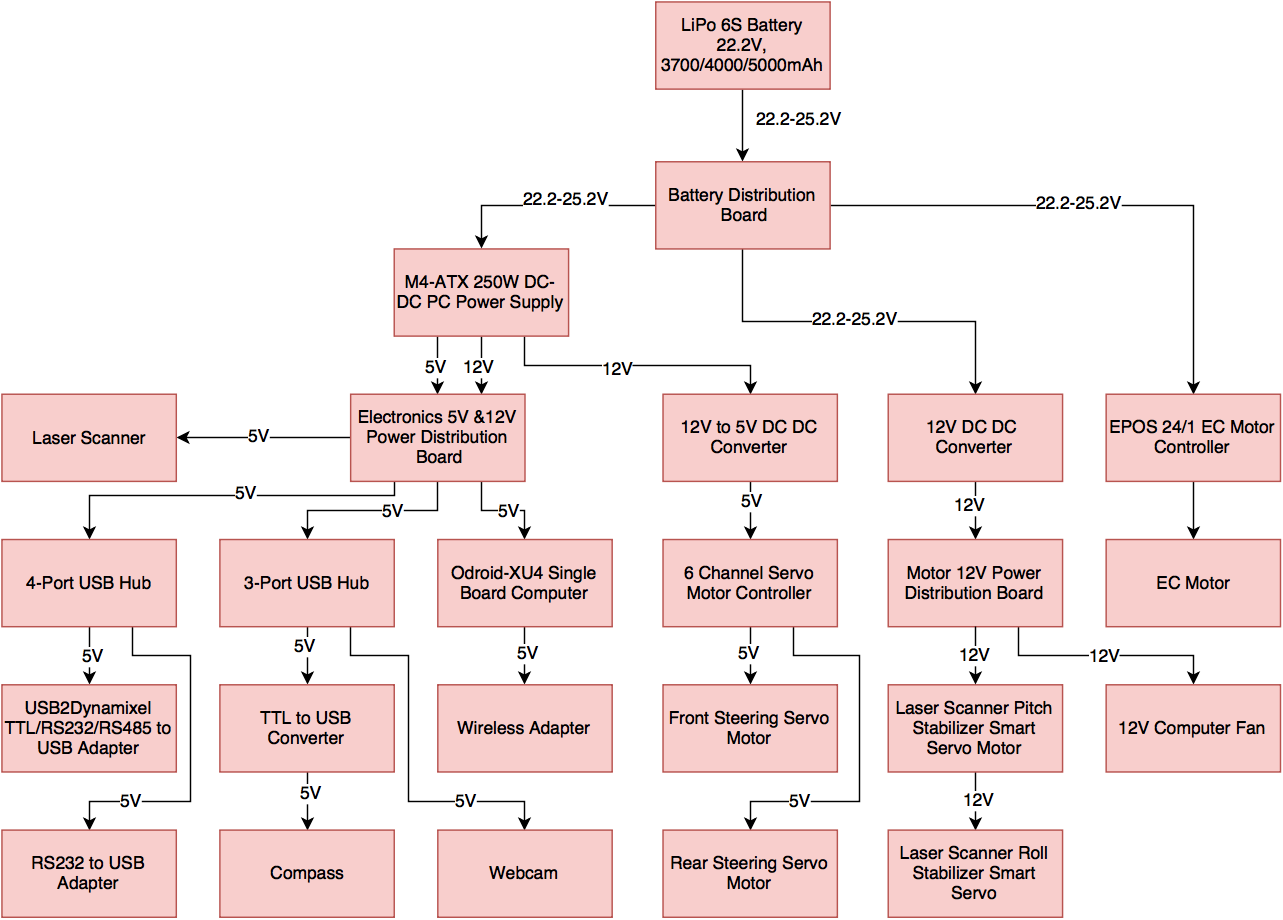
\includegraphics[width=0.9\linewidth]{Chapters/Chapter2/Figures/power_distribution.png}
	\caption{Σύστημα Τροφοδοσίας της ρομποτικής πλατφόρμας \textit{Monstertruck}.}
	\label{fig:power_distribution}
\end{figure}


%%%%%%%%%%%%%%%%%%%%%%%%%%%%%%%%%%%%%%%%%%%%%%%%%%%%%%%%%%%%%%%%%%%%%%%%%%%%%%%%%%%%%%%%%%%%
%\bigskip
%\subsubsection{Χωροθέτηση Υποσυστημάτων Ρομποτικής Πλατφόρμας \textit{Monstertruck}} ???
%%%%%%%%%%%%%%%%%%%%%%%%%%%%%%%%%%%%%%%%%%%%%%%%%%%%%%%%%%%%%%%%%%%%%%%%%%%%%%%%%%%%%%%%%%%%

%%%%%%%%%%%%%%%%%%%%%%%%%%%%%%%%%%%%%%%%%%%%%%%%%%%%%%%%%%%%%%%%%%%%%%%%%%%%%%%%%%%%%%%%%%%%%%
%%%%%%%%%%%%%%%%%%%%%%%%%%%%%%%%%%%%%%%%%%%%%%%%%%%%%%%%%%%%%%%%%%%%%%%%%%%%%%%%%%%%%%%%%%%%%%
%%%%%%%%%%%%%%%%%%%%%%%%%%%%%%%%%%%%%%%%%%%%%%%%%%%%%%%%%%%%%%%%%%%%%%%%%%%%%%%%%%%%%%%%%%%%%%

%----------------------------------------------------------------------------------------
%	SECTION 2: Motion Transfer System
%----------------------------------------------------------------------------------------
\newpage
\section{Σύστημα Μετάδοσης Κίνησης} \label{sec:motion_transfer_system}
Ένα αυτοκίνητο όχημα, για να κινηθεί, απαιτεί την ύπαρξη \textit{ενεργοποιητών(actuators)}, οι οποίοι μετατρέπουν την ενέργεια από μία πηγή τροφοδοσίας και ένα σήμα ελέγχου σε μηχανική κίνηση. Τον σκοπό αυτό, εξυπηρετούν οι κινητήρες και στην προκειμένη περίπτωση, για την επίτευξη της μηχανικής κίνησης του υλοποιημένου ρομποτικού οχήματος, χρησιμοποιούνται ένας κινητήρας, ο οποίος, μέσω ενός συστήματος μετάδοσης κίνησης, μεταδίδει την περιστροφική κίνηση του και στους τέσσερις τροχούς του οχήματος (\textit{τετρακίνηση}) και δύο σερβοκινητήρες, οι οποίοι στρίβουν και τους τέσσερις τροχούς, με ανεξάρτητη στρέψη των μπροστινών, από τους πίσω τροχούς  (\textit{τετραδιεύθυνση}). Στην συνέχεια, παρουσιάζεται η ανάλυση των μηχανισμών \textit{τετρακίνησης} και \textit{τετραδιεύθυνσης} της ρομποτικής πλατφόρμας \textit{Monstertruck}.


\bigskip
\subsection{Σύστημα Τετρακίνησης} \label{ssec:four_wheel_drive}
Η μετάδοση της κίνησης, από τον μοναδικό κινητήρα του οχήματος, προς τους τέσσερις τροχούς, δηλαδή η τετρακίνηση επιτυγχάνεται, μέσω του \textit{συστήματος μετάδοσης κίνησης (drivetrain)}, όπως φαίνεται στο σχήμα \ref{fig:drivetrain}. Το σύστημα αυτό περιλαμβάνει, συνολικά τέσσερα στάδια μετάδοσης της περιστροφικής κίνησης του κινητήρα, προς κάθε τροχό, όπου κάθε στάδιο εισάγει ένα λόγο μείωσης των στροφών, αλλά ταυτόχρονα, αντίστοιχο λόγο αύξησης της ροπής στρέψης.

\bigskip
\begin{figure}[!ht]
	\centering
	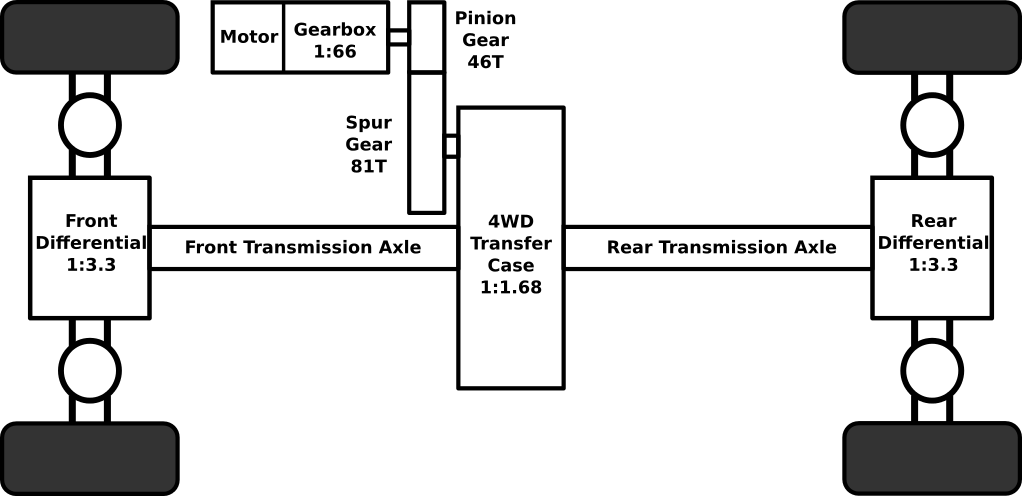
\includegraphics[width=0.8\linewidth]{Chapters/Chapter2/Figures/drivetrain.png}
	\caption{Σύστημα Μετάδοσης Κίνησης (Drivetrain) της ρομποτικής πλατφόρμας \textit{Monstertruck.}}
	\label{fig:drivetrain}
\end{figure}

\bigskip
Το πρώτο στάδιο, αποτελεί το \textit{κιβώτιο ταχυτήτων - μειωτήρας (gearbox)} του κινητήρα, το οποίο περιγράφεται από ένα λόγο μετάδοσης $\lambda_{gearbox}=1:66$. Ο λόγος, αυτός, μειώνει την μέγιστη περιστροφική ταχύτητα του κινητήρα, από $18\,000rpm$ σε $18\,000:66=272.72rpm$.

\bigskip
Το δεύτερο στάδιο μετάδοσης, αποτελείται από δύο γρανάζια, το \textit{Πινιόν (Pinion Gear)} και \textit{Ώθησης (Spur Gear)}. Το \textit{γρανάζι Πινιόν}, μεταδίδει την κίνηση από τον κινητήρα στο \textit{γρανάζι Ώθησης}, το οποίο, με τη σειρά του μεταδίδει την κίνηση στο επόμενο στάδιο μετάδοσης. Το \textit{γρανάζι Πινιόν} περιλαμβάνει $46$ οδοντώσεις, ενώ το \textit{γρανάζι Ώθησης}, $81$, έχοντας ως αποτέλεσμα ένα λόγο μετάδοσης $\lambda_{spur\_pinion}=46:81=1:1.76$. Με την μείωση του δεύτερου σταδίου, η μέγιστη ταχύτητα μειώνεται στα $272.72:1.76 = 154.96rpm$.

\begin{figure}[!ht]
	\centering
	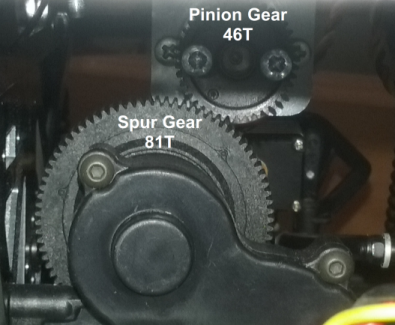
\includegraphics[width=0.4\linewidth]{Chapters/Chapter2/Figures/spur_and_pinion_gears.png}
	\caption{Γρανάζια Πινιόν και Ώθησης.}
	\label{fig:spur_pinion_gears}
\end{figure}

\bigskip
Το τρίτο στάδιο μετάδοσης και σημαντικότερο, για την επίτευξη \textit{τετρακίνησης}, περιλαμβάνει το \textit{κιβώτιο μετάδοσης (Transfer Case)} του μπροστινού και του πίσω άξονα, που φαίνεται στο σχήμα \ref{fig:transfer_case}. Το \textit{κιβώτιο μετάδοσης}, περιλαμβάνει δύο γρανάζια, το \textit{γρανάζι μετάδοσης (Transmission Gear)} και το \textit{διαφορικό γρανάζι (Differential Gear)}. Η περιστροφική κίνηση μεταδίδεται, από το \textit{γρανάζι Ώθησης}, προς το \textit{γρανάζι μετάδοσης}, μέσω ενός μηχανισμού \textit{σφιγκτήρα ολίσθησης (slipper clutch)}, που επιτρέπει την αποσύμπλεξη των γραναζιών, μέσω ολίσθησης, σε περίπτωση, υψηλής ροπής στους τροχούς, που θα μπορούσαν να προκαλέσουν ζημιά στα γρανάζια και στους άξονες μετάδοσης. Υπό φυσιολογικές συνθήκες, το \textit{γρανάζι μετάδοσης}, μεταδίδει την περιστροφική κίνηση προς το \textit{διαφορικό γρανάζι} και έπειτα προς τους δύο άξονες μετάδοσης, με λόγο μετάδοσης $\lambda_{transfer\_case}=1:1.68$. Επομένως, έχουμε μία επιπλέον μείωση των στροφών, με αποτέλεσμα $154.96:1.68=92.24rpm$.

\begin{figure}[!ht]
	\centering
	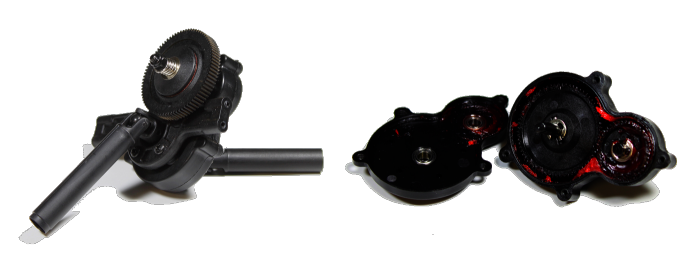
\includegraphics[width=0.8\linewidth]{Chapters/Chapter2/Figures/transfer_case.png}
	\caption{To κιβώτιο μετάδοσης κίνησης (Transfer Case) του οχήματος GroundPounder.}
	\label{fig:transfer_case}
\end{figure}

\bigskip
Το τέταρτο και τελευταίο στάδιο μετάδοσης της κίνησης, αποτελείται από δύο \textit{διαφορικά (differential)}, ένα για τους μπροστινούς τροχούς και ένα για τους πίσω. Το \textit{διαφορικό} είναι ένας μηχανισμός, ο οποίος μετατρέπει την κατεύθυνση κίνησης, από την ευθύγραμμη, του άξονα μετάδοσης, στην εγκάρσια, των ημιαξόνων κάθε τροχού. Παράλληλα, επιτρέπει σε δύο τροχούς, έναν αριστερό και ένα δεξιό, να κινούνται με διαφορετική περιστροφική ταχύτητα ή ροπή, ανάλογα με την πρόσφυση σε κάθε έναν, από αυτούς. Ο μηχανισμός, αυτός, είναι απαραίτητος, καθώς, όταν ένα όχημα προσπαθεί να στρίψει, ακολουθώντας μία καμπύλη, οι τροχοί που βρίσκονται στην εξωτερική πλευρά της καμπύλης, διανύουν μεγαλύτερη απόσταση, από τους εσωτερικούς τροχούς και άρα θα πρέπει να κινούνται με μεγαλύτερη ταχύτητα. Τέλος, το κάθε \textit{διαφορικό} εισάγει, ακόμη, έναν τελευταίο λόγο μείωσης των στροφών, της τάξης του $\lambda_{differential}=1:3.3$, οπότε η τελική μέγιστη ταχύτητα περιστροφής των τροχών προκύπτει $92.24:3.3=27.95rpm$.

\begin{figure}[!ht]
	\begin{minipage}{.49\textwidth}
		\centering
		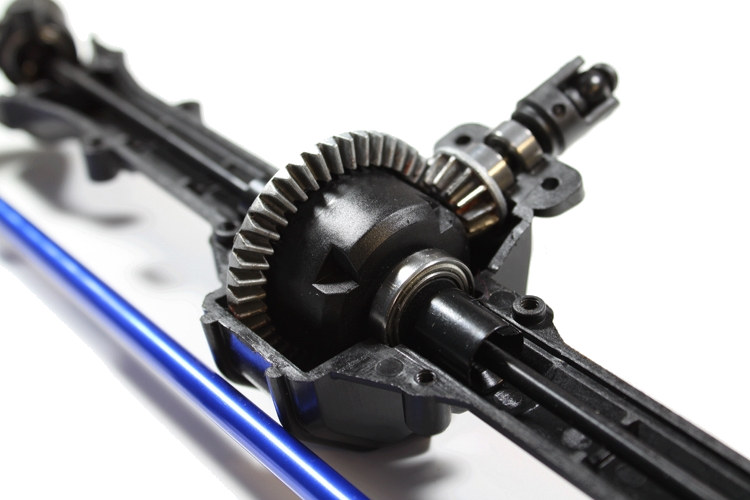
\includegraphics[width=0.5\linewidth]{Chapters/Chapter2/Figures/differential.png}
		\captionof{figure}{Το διαφορικό (Differential) του οχήματος GroundPounder.}
		\label{fig:differential}
	\end{minipage}
	\begin{minipage}{.5\textwidth}
	 	\centering		
		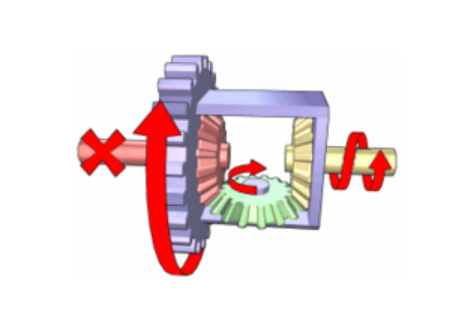
\includegraphics[width=0.5\linewidth]		
			{Chapters/Chapter2/Figures/differential_function.png}
		\captionof{figure}{Λειτουργία ενδεικτικού μηχανισμού διαφορικού.}
		\label{fig:differential_function}
	\end{minipage}
\end{figure}

\bigskip
Επομένως, η σχέση μετάδοσης της περιστροφικής ταχύτητας, από τον κινητήρα, στους τροχούς προκύπτει:

\begin{equation}
	\omega_{wheel} = \omega_{motor} / (\lambda_{gearbox} \times \lambda_{spur\_pinion} \times \lambda_{transfer\_case} \times \lambda_{differential}) = \omega_{motor} / 644
\end{equation}

\bigskip
\subsection{Σύστημα Τετραδιεύθυνσης} \label{ssec:four_wheel_steering}
Η ρομποτική πλατφόρμα \textit{Monstertruck}, περιλαμβάνει δύο σερβοκινητήρες, υπεύθυνους για την ανεξάρτητη στρέψη των μπροστινών και πίσω τροχών. Η ανεξάρτητη αυτή στρέψη, επιτρέπει στο όχημα να λειτουργεί με μπροστινή στρέψη (\textit{Μπροστινοδιεύθυνση - FWS}), πίσω στρέψη (\textit{Πίσωδιεύθυνση - RWS}), ή ταυτόχρονη στρέψη (\textit{Τετραδιεύθυνση - 4WS}) των τροχών. Στην \textit{τετραδιεύθυνση}, οι μπροστινοί τροχοί, μπορεί να στρίβουν, είτε, με την ίδια φορά με τους πίσω τροχούς, οπότε μιλάμε για \textit{θετική τετραδιεύθυνση}, είτε με αντίθετη, οπότε μιλάμε για \textit{αρνητική τετραδιεύθυνση}.

\bigskip
Εφόσον, υπάρχει ένας σερβοκινητήρας, για τους μπροστινούς τροχούς και ένας για τους πίσω, γεννάται το ερώτημα, πώς μεταδίδεται η στρέψη από έναν σερβοκινητήρα σε δύο τροχούς, έναν αριστερό και έναν δεξιό. Ο μηχανισμός, που λύνει το πρόβλημα, στην προκειμένη περίπτωση, ονομάζεται \textit{Μηχανισμός Στρέψης, μέσω Συνδέσμου Έλξης (Drag Link Steering Mechanism)}. Ο  μηχανισμός αυτός, στην προκειμένη περίπτωση, αποτελείται από έναν σερβοκινητήρα, ένα \textit{μπράτσο Pitman (Pitman Arm)}, έναν \textit{σύνδεσμο έλξης (Drag Link)} και έναν \textit{σύνδεσμο ένωσης των τροχών (Tie Rod)}, όπως επίσης και τις \textit{αρθρώσεις στρέψης των τροχών (Wheel Steering Knuckles)}, όπως και παρουσιάζεται στο σχήμα \ref{fig:drag_link_steering}.

\begin{figure}[!ht]
	\centering
	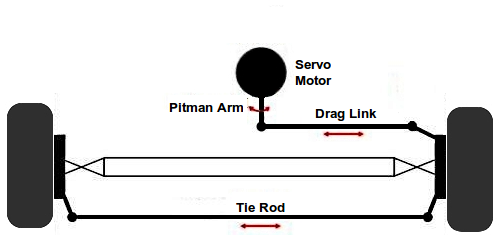
\includegraphics[width=0.6\linewidth]{Chapters/Chapter2/Figures/my_drag_link_steering.png}
	\caption{Ο Μηχανισμός στρέψης, με άξονα έλξης (Drag Link Steering Mechanism)
	\\της ρομποτικής πλατφόρμας Monstertruck.}
	\label{fig:drag_link_steering}
\end{figure}

\bigskip
Η περιστροφική κίνηση του σερβοκινητήρα, μεταδίδεται μέσω του \textit{μπράτσου Pitman} και μετατρέπεται σε μεταφορική κίνηση του \textit{συνδέσμου έλξης}, η οποία με τη σειρά της μετατρέπεται σε στρέψη της άρθρωσης του δεξιού τροχού. Η στρέψη, τώρα, της δεξιάς άρθρωσης, παρασύρει τον \textit{σύνδεσμο ένωσης} των αρθρώσεων στρέψης των τροχών σε μεταφορική κίνηση, η οποία, έχει σαν αποτέλεσμα την στρέψη και του αριστερού τροχού. Ακολούθως, αναλύεται η λειτουργία του μηχανισμού στρέψης, σε δύο βήματα. Πρώτα υπολογίζεται η μετατόπιση $\Delta x$ του \textit{συνδέσμου έλξης}, συναρτήσει της γωνίας στρέψης $\theta$ του σερβοκινητήρα και έπειτα, συναρτήσει της γωνίας στρέψης $\delta$ της άρθρωσης τροχού, με την οποία, είναι συνδεδεμένος ο \textit{σύνδεσμος έλξης}.

\bigskip
\begin{figure}[!ht]
	\centering
	\subfloat[Ανάλυση για $\theta < 0$.]{
	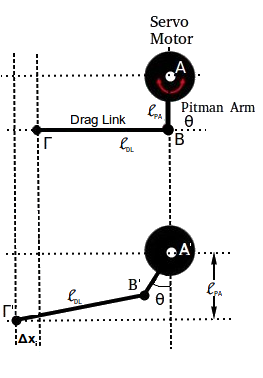
\includegraphics[width=0.4\linewidth]{Chapters/Chapter2/Figures/drag_link_analysis_1.png}
	\label{fig:drag_link_analysis_a}}
	\centering
	\subfloat[Ανάλυση για $\theta > 0$.]{
	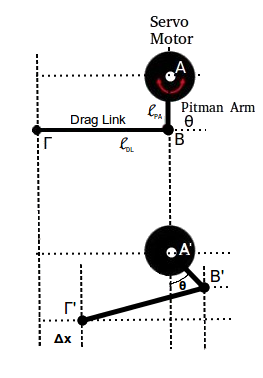
\includegraphics[width=0.4\linewidth]{Chapters/Chapter2/Figures/drag_link_analysis_2.png}
	\label{fig:drag_link_analysis_b}}
	\caption{Μετάδοση κίνησης από τον σερβοκινητήρα και το μπράτσο Pitman στον σύνδεσμο έλξης.}
	\label{fig:drag_link_analysis}	
\end{figure}

\bigskip
Λαμβάνοντας την παραδοχή, ότι η άκρη (σημείο Γ) του συνδέσμου έλξης, κινείται, μόνο οριζόντια και όχι κάθετα και με βάση το σχήμα \ref{fig:drag_link_analysis} και απλή γεωμετρική ανάλυση, μπορεί να εξαχθεί η  σχέση μεταξύ της γωνίας στρέψης $\theta$ του σερβοκινητήρα και της μετατόπισης $\Delta x$ του \textit{συνδέσμου έλξης}, ως:

\begin{equation}
	\label{eq:drag_link_displacement}
	\Delta x =
	\begin{cases}
		\sqrt{l_{DL}^2 - l_{PA}^2(1-\cos(\theta))^2} + l_{PA} \sin(|\theta|) - l_{DL},  &\theta < 0\\ \\
	0, &\theta = 0\\ \\ 
	-\sqrt{l_{DL}^2 - l_{PA}^2(1-\cos(\theta))^2} - l_{PA} \sin(|\theta|) - l_{DL}, &\theta > 0
	\end{cases}
\end{equation}

\bigskip\noindent
όπου $l_{DL}$ είναι το μήκος του \textit{συνδέσμου έλξης} και $l_{PA}$ είναι το μήκος του \textit{μπράτσου Pitman}.

\begin{figure}[!ht]
	\centering
	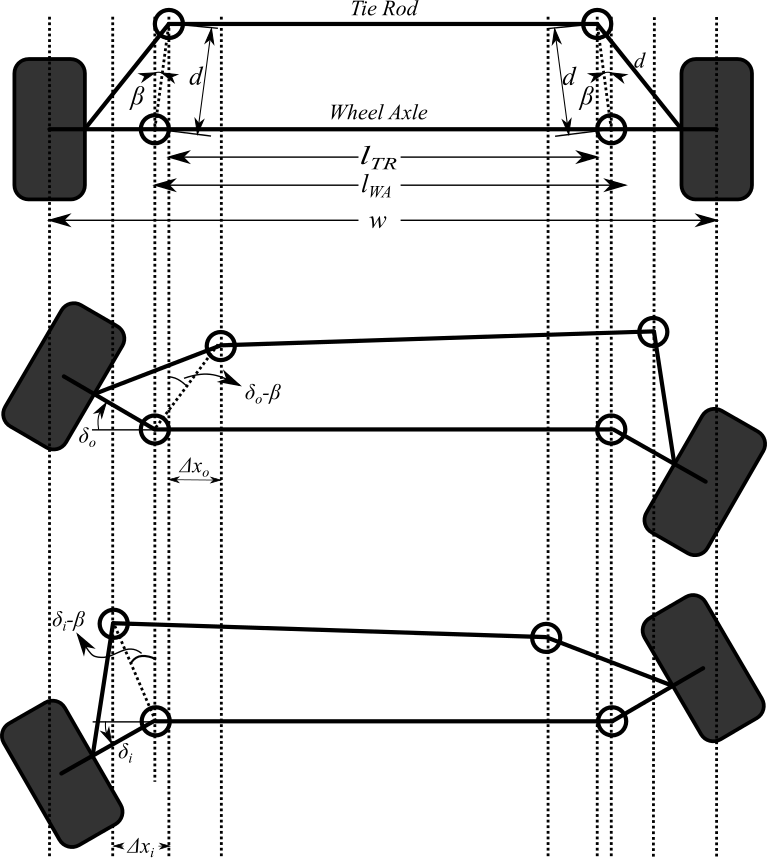
\includegraphics[width=0.8\linewidth]{Chapters/Chapter2/Figures/trapezoid_steering_mechanism.png}
	\caption{Τραπεζοειδής Μηχανισμός στρέψης των τροχών.}
	\label{fig:trapezoid_steering_mechanism}
\end{figure}

\bigskip
Με βάση το σχήμα \ref{fig:trapezoid_steering_mechanism}, μέσω γεωμετρικής ανάλυσης, προκύπτει ότι, η μετατόπιση του \textit{συνδέσμου έλξης} $\Delta x$, συναρτήσει της γωνίας στρέψης, του άμεσα συνδεδεμένου τροχού, δηλαδή του αριστερού, στην προκειμένη περίπτωση, για τις περιπτώσεις, που ο τροχός είναι στην εσωτερική ή στην εξωτερική  πλευρά της στροφής, λαμβάνεται μέσω των ακόλουθων σχέσεων.
 
\begin{align}
	\label{eq:tie_rod_inner_displacement}
	\Delta x_i = d \sin(\delta_i - \beta) + d \sin(\beta)\\
	\label{eq:tie_rod_outer_displacement}\\
	\Delta x_o = d \sin(\delta_o + \beta) - d \sin(\beta)
\end{align}

\bigskip
Εξισώνοντας, τώρα, τις σχέσεις (\ref{eq:drag_link_displacement}), (\ref{eq:tie_rod_inner_displacement}), (\ref{eq:tie_rod_outer_displacement}), προκύπτει η σχέση μεταξύ της γωνίας στρέψης του σερβοκινητήρα και της γωνίας στρέψης του αριστερού τροχού, για τις περιπτώσεις που είναι εσωτερικά ($\delta_i$) στην στροφή και εξωτερικά ($\delta_o$):

\begin{equation}
	\label{eq:inner_steering_angle}
	\delta_i = \beta + \sin^{-1}{ \Bigg(
		\frac{
		\sqrt{l_{DL}^2 - l_{PA}^2(1-\cos(\theta))} + l_{PA} \sin{|\theta|} - l_{DL} - d \sin{\beta}}{d}} \Bigg)
\end{equation}

\begin{equation}
	\label{eq:outer_steering_angle}
	\delta_o = -\beta + \sin^{-1}{ \Bigg(
		\frac{
		-\sqrt{l_{DL}^2 - l_{PA}^2(1-\cos(\theta))} - l_{PA} \sin{|\theta|} - l_{DL} + d \sin{\beta}}{d}} \Bigg)
\end{equation}

\bigskip
Ο υπολογισμός της γωνίας στρέψης, του απέναντι τροχού, δηλαδή, στην προκειμένη περίπτωση, του δεξιού τροχού, προκύπτει από τις εξισώσεις \textit{τραπεζοειδούς μηχανισμού στρέψης τροχών} \cite{vehicle_dynamics}:

\begin{equation}
	\label{eq:trapezoid_steering_mechanism}
	sin(\beta + \delta_i) + sin(\beta - \delta_o) = \frac{L}{d} + \sqrt{\big(\frac{L}{d} - w \sin{\beta} \big)^2 - \big(\cos{(\beta-\delta_o)} - \cos{(\beta+\delta_i)}\big)^2}
\end{equation}

\bigskip
Αντικαθιστώντας την τιμή για την $\delta_i$, στην εξίσωση (\ref{eq:trapezoid_steering_mechanism}) θα πρέπει να εφαρμοστεί, ένας επαναληπτικός αλγόριθμος, για την εύρεση της $\delta_o$ και αντίστροφα.

\bigskip
Για την απλοποίηση της όλης διαδικασίας μετατροπής της γωνίας στρέψης του σερβοκινητήρα, σε γωνίες στρέψης των τροχών και αντίστροφα, χρησιμοποιήθηκαν πολυωνυμικές προσεγγίσεις των σχέσεων μεταξύ αυτών, λύνοντας, επαναληπτικά και για όλες τις δυνατές τιμές, τις εξισώσεις (\ref{eq:inner_steering_angle}), (\ref{eq:outer_steering_angle}), (\ref{eq:trapezoid_steering_mechanism}) και για τις τιμές των παραμέτρων του μηχανισμού στρέψης που φαίνονται στον πίνακα \ref{tab:steering_parameter_values}.

\bigskip
\begin{table}[!ht]
	\centering
	\captionof{table}{Παράμετροι του μηχανισμού μετάδοσης στρέψης των τροχών.}
	\begin{tabular}{| l | c |}
		\hline
		\textbf{Παράμετρος} & \textbf{Τιμή}\\ \hline
		$d$ & $30mm$ \\ \hline
		$\beta$ & $5^\circ$\\ \hline
		$l_{TR}$ & $225mm$\\ \hline
		$l_{WA}$ & $230mm$\\ \hline
		$l_{PA}$ & $20mm$\\ \hline
		$l_{DA}$ & $100mm$\\ \hline
	\end{tabular}
	\label{tab:steering_parameter_values}
\end{table}

%\begin{align}
%\begin{split}
%	\delta_{LF} &= -0.0082\;\cdot \theta_{F}^5 - 0.0162\;\cdot \theta_{F}^4 - 0.00605\;\cdot \theta_{F}^3 - 0.0192\;\cdot \theta_{F}^2 + 0.6691\;\cdot \theta_{F}\\
%	\delta_{LR} &= 0.0082\;\cdot \theta_{R}^5 + 0.0162\;\cdot \theta_{R}^4 + 0.00605\;\cdot \theta_{R}^3 + 0.0192\;\cdot \theta_{R}^2 - 0.6691\;\cdot \theta_{R}\\
%	\delta_{RF} &= 0.0126\;\cdot \delta_{LF}^5 - 0.0432\;\cdot \delta_{LF}^4 + 0.0067\;\cdot \delta_{LF}^3 - 0.0851\;\cdot \delta_{LF}^2 + 0.9997\;\cdot \delta_{LF} + 0.0035\\
%	\delta_{RR} &= -0.0126\;\cdot \delta_{LR}^5 + 0.0432\;\cdot \delta_{LR}^4 - 0.0067\;\cdot \delta_{LR}^3 + 0.0851\;\cdot \delta_{LR}^2 - 0.9997\;\cdot \delta_{LR} - 0.0035\\
%	\theta_{F} &= 0.5334\;\cdot \delta_{LF}^5 + 0.2997\;\cdot \delta_{LF}^4 + 0.2857\;\cdot \delta_{LF}^3 + 0.0556\;\cdot \delta_{LF}^2 + 1.4951\;\cdot \delta_{LF}\\
%	\theta_{R} &= - 0.5334\;\cdot \delta_{LR}^5 - 0.2997\;\cdot \delta_{LR}^4 - 0.2857\;\cdot \delta_{LR}^3 - 0.0556\;\cdot \delta_{LR}^2 - 1.4951\;\cdot \delta_{LR}\\
%\end{split}
%\end{align}

\begin{align}
\begin{split}
\delta_{lf} &= -0.029\;\cdot \theta_{f}^2 - 0.6515\;\cdot \theta_{f} - 0.0006\\
\delta_{lr} &= 0.029\;\cdot \theta_{r}^2 + 0.6515\;\cdot \theta_{r} + 0.0006\\
\delta_{rf} &= -0.0058\;\cdot \delta_{lf}^2 + 1.0203\;\cdot \delta_{lf}\\
\delta_{rr} &= 0.0058\;\cdot \delta_{lr}^2 - 1.0203\;\cdot \delta_{lr}\\
\theta_{f}\, &= 0.1047\;\cdot \delta_{lf}^2 + 1.5362\;\cdot \delta_{lf} + -0.0009\\
\theta_{r}\, &= -0.1047\;\cdot \delta_{lr}^2 - 1.5362\;\cdot \delta_{lr} - 0.0009
\end{split}
\label{eq:polynoms}
\end{align}

\bigskip
\noindent
όπου

\begin{description}
	\item[\theta_{f}:] γωνία στρέψης του μπροστινού σερβοκινητήρα
	\item[\theta_{r}:] γωνία στρέψης του πίσω σερβοκινητήρα
	\item[\delta_{lf}:] γωνία στρέψης του μπροστινού αριστερού τροχού
	\item[\delta_{lr}:] γωνία στρέψης του πίσω αριστερού τροχού
	\item[\delta_{rf}:] γωνία στρέψης του μπροστινού δεξιού τροχού
	\item[\delta_{rr}:] γωνία στρέψης του πίσω δεξιού τροχού
\end{description}

%%%%%%%%%%%%%%%%%%%%%%%%%%%%%%%%%%%%%%%%%%%%%%%%%%%%%%%%%%%%%%%%%%%%%%%%%%%%%%%%%%%%%%%%%%%%%%
%%%%%%%%%%%%%%%%%%%%%%%%%%%%%%%%%%%%%%%%%%%%%%%%%%%%%%%%%%%%%%%%%%%%%%%%%%%%%%%%%%%%%%%%%%%%%%
%%%%%%%%%%%%%%%%%%%%%%%%%%%%%%%%%%%%%%%%%%%%%%%%%%%%%%%%%%%%%%%%%%%%%%%%%%%%%%%%%%%%%%%%%%%%%%

%----------------------------------------------------------------------------------------
%	SECTION 3: Kinematic Analysis
%----------------------------------------------------------------------------------------
\bigskip
\section{Κινηματική Ανάλυση} \label{sec:kinematic_analysis}
Ένα σύγχρονο αυτοκίνητο όχημα, στην πλειονότητα των περιπτώσεων, για να κινηθεί, περιλαμβάνει έναν κινητήρα, ο οποίος είναι υπεύθυνος για την περιστροφική κίνηση των μπροστινών (μπροστινοκίνηση), πίσω (πισωκίνηση) ή όλων (τετρακίνηση) των τροχών. Επίσης, περιλαμβάνει ένα σύστημα στρέψης των τροχών, είτε μπροστινών (μπροστινοδιεύθυνση), είτε πισινών (πισωδιεύθυνση), είτε και των τεσσάρων (τετραδιεύθυνση), έτσι ώστε να μπορεί να ακολουθεί καμπύλες τροχιές και όχι μόνο ευθύγραμμες. Η κινηματική ανάλυση του οχήματος, που παρουσιάζεται στην παρούσα ενότητα, προσπαθεί να περιγράψει την επίδραση του ελέγχου κίνησης των τροχών του, στην κίνηση του οχήματος και στις μεταβολές της \textit{κατάστασης} του.

\bigskip
Η \textit{κατάσταση} ενός άκαμπτου (rigid) ρομποτικού οχήματος, συνήθως περιγράφεται, από έξι μεταβλητές, τις καρτεσιανές συντεταγμένες του x, y, z, ως προς ένα αυθαίρετο εξωτερικό σύστημα συντεταγμένων και τις \textit{γωνίες Euler yaw, pitch, roll}. Στην προκειμένη περίπτωση, το πρόβλημα που εξετάζεται, περιορίζεται σε επίπεδο περιβάλλον και επομένως, ως \textit{κατάσταση} του οχήματος, λαμβάνεται, η \textit{πόζα} του $\mathbf{q}$, η οποία περιγράφεται από τις καρτεσιανές συνταγμένες του $x, y$ στο επίπεδο και τον προσανατολισμό του $\theta$, ως προς αυθαίρετο εξωτερικό σύστημα συντεταγμένων.

\begin{equation}
	\textbf{q} = [x\;\; y\;\; \theta]^T
	\label{eq:pose}
\end{equation}

\bigskip
Αντίστοιχα, η ταχύτητα ενός ρομποτικού οχήματος στο επίπεδο, ως προς ένα αυθαίρετο εξωτερικό σύστημα συντεταγμένων ορίζεται ως η μεταβολή της \textit{πόζας} του $\mathbf{q}$, ως προς τον χρόνο.

\begin{equation}
	\dot{\mathbf{q}} = [\dot x\;\; \dot y\;\; \dot \theta]^T
	\label{eq:dpose}
\end{equation}

\bigskip
\noindent
Ενώ, η ταχύτητα ενός ρομποτικού οχήματος, στο επίπεδο, ως προς το κέντρο μάζας του $C$ είναι

\begin{equation}
	 \textbf{v} = [v_{cx}\;\; v_{cy}\;\; \omega_c]^T
	\label{eq:speed}
\end{equation}

\bigskip
\noindent
και αντιστοιχεί σε μία κυκλική τροχιά, ακτίνας $R$. Εφόσον, ένα διάνυσμα ταχυτήτων, αντιστοιχεί σε μία κυκλική τροχιά του κέντρου μάζας $C$ του οχήματος, τότε, μία επιθυμητή καμπύλη τροχιά, μπορεί να προσεγγιστεί, από ένα σύνολο τόξων κύκλου και τις αντίστοιχες  ταχύτητες τους.

% Στην ειδική περίπτωση των οχημάτων, με \textit{κινηματικό Ackermann} ή \textit{κινηματικό Τετραδιεύθυνσης}, που εξετάζεται οι κυκλικές τροχιές - τόξα κύκλου, μπορούν να καθοριστούν πλήρως από τις γωνίες στρέψης των τροχών και ανεξάρτητα από την γραμμική ταχύτητα του οχήματος, σε αντίθεση με άλλα κινηματικά μοντέλα (differential, skid steer, holonomic). Με βάση, αυτήν την παρατήρηση, πραγματοποιείται, στην συνέχεια η κινηματική ανάλυση των μοντέλων \textit{Ackermann, Τετραδιεύθυνσης} και τελικά της υλοποιημένης ρομποτικής πλατφόρμας \textit{Monstertruck}.

\bigskip
\subsection{Κινηματικό Μοντέλο Ackermann} \label{ssec:ackermann_kinematics}
Το \textit{Κινηματικό Μοντέλο Ackermann}, αποτελεί το δημοφιλέστερο και πιο διαδεδομένο κινηματικό μοντέλο στην αυτοκινητοβιομηχανία. Αναπτύχθηκε από τον Γερμανό μηχανικό Georg Lankensperger στο Μόναχο, το 1817, αλλά το δίπλωμα ευρεσιτεχνίας κατοχυρώθηκε από τον Rudolph Ackermann, το 1818, για ιππήλατες άμαξες. Τελικά, επεκτάθηκε και στην αυτοκινητοβιομηχανία και χρησιμοποιείται μέχρι και σήμερα.

\bigskip 
Σκοπός του κινηματικού μοντέλου \textit{Ackermann} είναι η αποφυγή της πλευρικής ολίσθησης των τροχών, ενός τετράτροχου οχήματος κατά την ακολούθηση καμπύλων τροχιών. Για την εξυπηρέτηση αυτού του σκοπού, λοιπόν, το \textit{κινηματικό μοντέλο Ackermann}, στηρίζεται σε μία συνθήκη, την λεγόμενη \textit{συνθήκη Ackermann}, μεταξύ των τροχών στρέψης ενός οχήματος, που αν ικανοποιείται προβλέπει την κίνηση των τροχών, χωρίς πλευρική ολίσθηση \cite{vehicle_dynamics}. Η συνθήκη Ackermann, υποστηρίζει ότι για να κινείται ένα τετράτροχο όχημα χωρίς να ολισθαίνουν πλευρικά οι τροχοί του, θα πρέπει οι κάθετοι, στους τροχούς, άξονες να τέμνονται σε ένα κοινό σημείο, το οποίο ονομάζεται \textit{Στιγμιαίο Κέντρο Περιστροφής (Instantaneous Center of Rotation - ICR)} \cite{4ws_kinematics} και αποτελεί το κέντρο της στιγμιαίας κυκλικής τροχιάς που ακολουθεί το όχημα.

\begin{figure}[!ht]
	\centering
	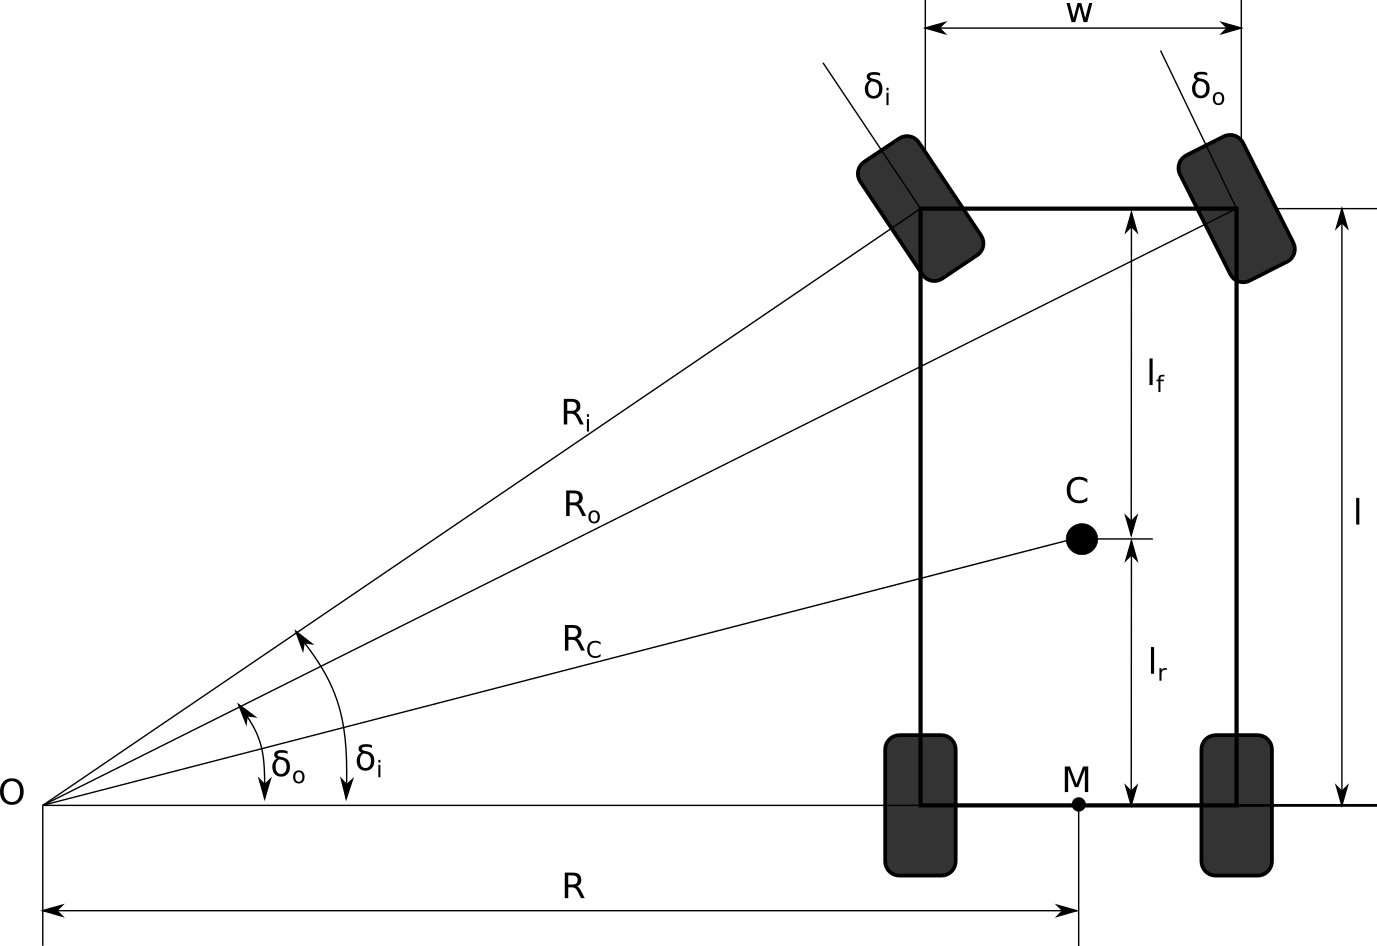
\includegraphics[width=0.7\linewidth]{Chapters/Chapter2/Figures/ackermann_model.png}
	\caption{Κινηματικό Μοντέλο Ackermann.}
	\label{fig:ackermann_model}
\end{figure}

\bigskip
Λαμβάνοντας υπόψιν το σχήμα \ref{fig:ackermann_model} προκύπτουν οι γωνίες στρέψης των τροχών ως

\begin{equation}
	\tan(\delta_i) = \frac{l}{R - \frac{w}{2}}
	\text{\;\;ή\;\;}	
	\cot(\delta_i) = \frac{R - \frac{w}{2}}{l}
	\label{eq:ackermann_inner_steering_angle}
\end{equation}

\begin{equation}
	\tan(\delta_o) = \frac{l}{R + \frac{w}{2}}
	\text{\;\;ή\;\;}
	\cot(\delta_o) = \frac{R + \frac{w}{2}}{l}
	\label{eq:ackermann_outer_steering_angle}
\end{equation}

Αφαιρώντας τις εξισώσεις (\ref{eq:ackermann_inner_steering_angle}), (\ref{eq:ackermann_outer_steering_angle}), προκύπτει η \textit{συνθήκη Ackermann}.

\begin{equation}
	\cot{\delta_i} - \cot{\delta_o} = w / l
	\label{eq:ackermann_condition}
\end{equation}


\noindent
όπου
\begin{description}
	\item[\delta_i:] γωνία στρέψης εσωτερικού (inner), ως προς την στροφή, τροχού.
	\item[\delta_o:] γωνία στρέψης εξωτερικού (outer), ως προς την στροφή, τροχού.
	\item[L:] μεταξόνιο (wheelbase).
	\item[w:] μετατρόχιο (track).
	\item[R:] ακτίνα τροχιάς που εκτελεί το μεσαίο σημείο μεταξύ των πίσω τροχών.
\end{description}

\bigskip
Το όχημα, που παρουσιάζεται στο σχήμα \ref{fig:ackermann_model}, πραγματοποιεί μία κυκλική τροχιά γύρω από το \textit{Στιγμιαίο Κέντρο Περιστροφής} Ο. Αν λάβοουμε ως σημείο αναφοράς το κέντρο του πίσω άξονα (σημείο $P$), τότε το όχημα εκτελεί μία κυκλική τροχιά, ακτίνας $R$, γύρω από το σημείο O. Η ακτίνα R, μπορεί να υπολογιστεί προσθέτοντας τις εξισώσεις (\ref{eq:ackermann_inner_steering_angle}), (\ref{eq:ackermann_outer_steering_angle}), ως

\begin{equation}
	R = l \cdot \frac{\cot{\delta_i} + \cot{\delta_o}}{2} = l \cot{\delta} = \frac{l}{\tan{\delta}}
	\label{eq:ackermann_rear_middle_turning_radius}
\end{equation}

\noindent
όπου $\delta$ είναι η γωνία στρέψης του ισοδύναμου κινηματικού μοντέλου ποδηλάτου (σχήμα \ref{fig:ackermann_bicylce_model}). 

\begin{figure}[!ht]
	\centering
	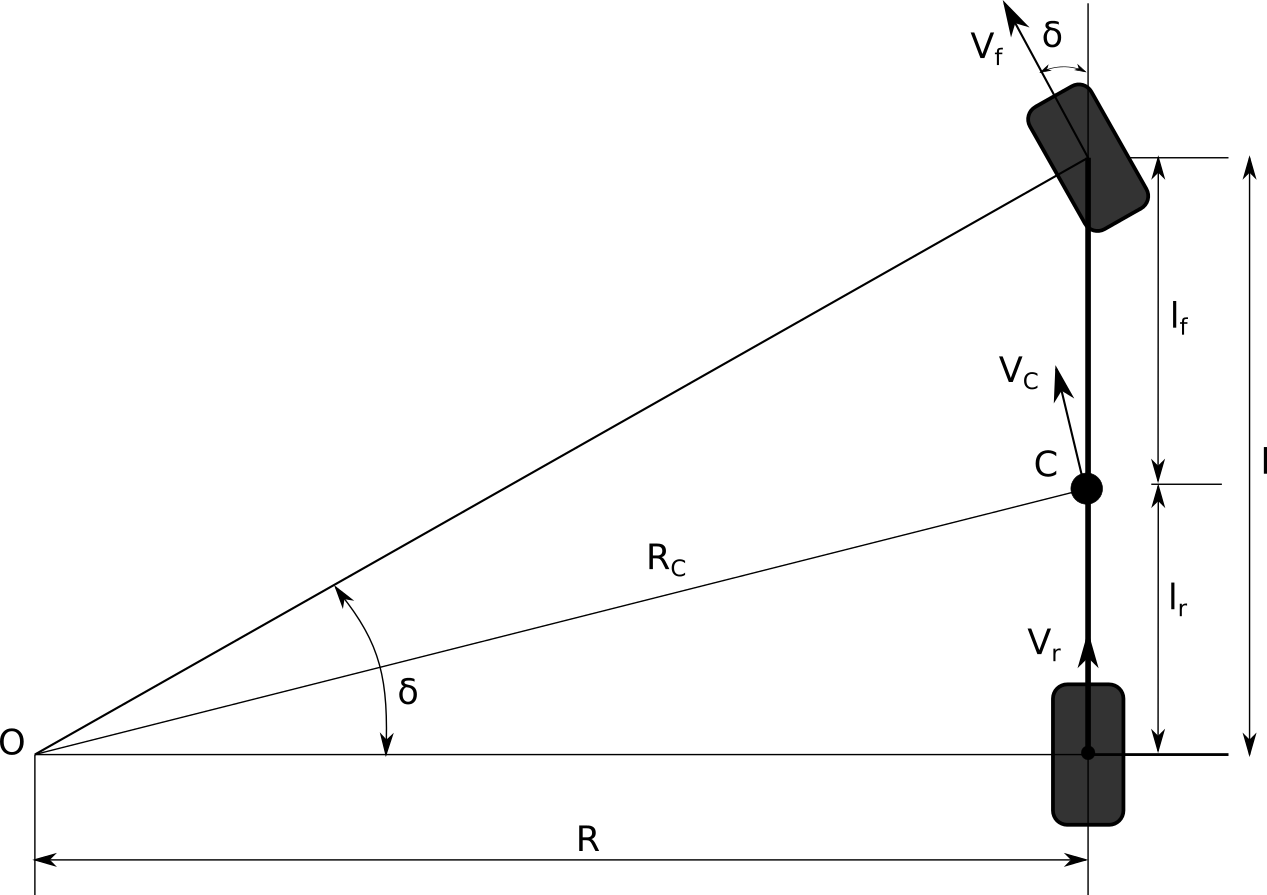
\includegraphics[width=0.6\linewidth]{Chapters/Chapter2/Figures/ackermann_bicycle_model.png}
	\caption{Ισοδύναμο μοντέλο ποδηλάτου Ackermann.}
	\label{fig:ackermann_bicylce_model}
\end{figure}

\bigskip
Αντίστοιχα, ο υπολογισμός της ακτίνας $R_c$ του κέντρου μάζας του οχήματος, με βάση το σχήμα \ref{fig:ackermann_model}, προκύπτει 

\begin{equation}
	R_c = \sqrt{R^2 + l_R^2} = \sqrt{R^2 + (l - l_F)^2}
	\label{eq:ackermann_center_mass_turning_radius}
\end{equation}

\noindent
όπου, $l_R$ και $l_F$ είναι η απόσταση του κέντρου μάζας του οχήματος από τον άξονα των μπροστινών και πίσω τροχών αντίστοιχα, όπου $l_R + l_F = l$.

\bigskip
Κατά την κίνηση σε κυκλική τροχιά, κάθε τροχός του οχήματος διαγράφει διαφορετική τροχιά από τους υπόλοιπους. Για παράδειγμα, στο σχήμα \ref{fig:ackermann_model}, για να καταστεί δυνατή η εκτέλεση της τροχιάς, γύρω από το Ο, χωρίς ολίσθηση, θα πρέπει οι τροχοί να κινούνται ίδια γωνιακή ταχύτητα $\dot\theta$, ως προς το κέντρο $O$ και με διαφορετική γραμμική ταχύτητα, και άρα, καθένας, να περιστρέφεται με διαφορετική περιστροφική ταχύτητα $\omega$, ανάλογη της ακτίνας της τροχιάς που διαγράφει. Επομένως, ισχύει

\begin{equation}
	\dot\theta_{ir} = \dot\theta_{or} = \dot\theta_{if} = \dot\theta_{of} = \dot\theta
	\label{eq:theta_dot}
\end{equation}

\bigskip
\noindent
και αντικαθιστώντας στην εξίσωση (\ref{eq:theta_dot}), την σχέση μεταξύ γωνιακής και γραμμικής ταχύτητας
	
\begin{equation}
	v = \dot\theta \cdot R
	\label{eq:v_theta}
\end{equation}	

\noindent
η εξίσωση (\ref{eq:theta_dot}) μετασχηματίζεται στη μορφή
	
\begin{equation}	
	\frac{v_{ir}}{R_{ir}} = \frac{v_{or}}{R_{or}} = \frac{v_{if}}{R_{if}} = \frac{v_{of}}{R_{of}} = \dot\theta = \frac{v_c}{R_c}
	\label{eq:theta_dot_2}
\end{equation}

\noindent
όπου
\begin{description}
	\item[ir:] εσωτερικός πίσω τροχός
	\item[or:] εξωτερικός πίσω τροχός
	\item[if:] εσωτερικός μπροστινός τροχός
	\item[of:] εξωτερικός μπροστινός τροχός
\end{description}

\bigskip
Επομένως, με βάση τις δύο παραπάνω παρατηρήσεις, και την σχέση (\ref{eq:theta_dot_2}) μπορεί να υπολογιστεί η γραμμική ταχύτητα κάθε τροχού, ως

\begin{align}
	v_{if} &= \dot\theta \cdot R_{if} = \dot\theta \cdot \sqrt{l^2 + (R - \frac{w}{2})^2}
	\label{eq:ack_vif}\\
	v_{of} &= \dot\theta \cdot R_{of} = \dot\theta \cdot \sqrt{l^2 + (R + \frac{w}{2})^2}
	\label{eq:ack_vof}\\
	v_{ir} &= \dot\theta \cdot R_{ir} = \dot\theta \cdot (R - \frac{w}{2})
	\label{eq:ack_vir}\\
	v_{or} &= \dot\theta \cdot R_{or} = \dot\theta \cdot (R + \frac{w}{2})
	\label{eq:ack_vor}
\end{align}

\bigskip
Χρησιμοποιώντας, τις εξισώσεις (\ref{eq:ack_vif}) - (\ref{eq:ack_vor}), όπως επίσης και την σχέση μεταξύ γραμμικής ταχύτητας $v$, περιστροφικής ταχύτητας $\omega$ και ακτίνας τροχού $r$
\begin{equation}
	v = \omega \cdot r
	\label{eq:v_omega}
\end{equation}

\noindent
προκύπτουν οι περιστροφικές ταχύτητες των τροχών, ως

\begin{align}
	\omega_{ir} &= \frac{\dot\theta}{r} \cdot R_{ir} = \frac{\dot\theta}{r} \cdot (R - \frac{w}{2})
	\label{eq:ack_wir}\\
	\omega_{or} &= \frac{\dot\theta}{r} \cdot R_{or} = \frac{\dot\theta}{r} \cdot (R + \frac{w}{2})
	\label{eq:ack_wor}\\
	\omega_{if} &= \frac{\dot\theta}{r} \cdot R_{if} = \frac{\dot\theta}{r} \cdot \sqrt{l^2 + (R - \frac{w}{2})^2}
	\label{eq:ack_wif}\\
	\omega_{of} &= \frac{\dot\theta}{r} \cdot R_{of} = \frac{\dot\theta}{r} \cdot \sqrt{l^2 + (R + \frac{w}{2})^2}
	\label{eq:ack_wof}
\end{align}

\bigskip
Τέλος, οι ταχύτητες του κέντρου του άξονα των πίσω τροχών, ως προς ένα αυθαίρετο εξωτερικό σύστημα συντεταγμένων, βάση του \textit{ισοδύναμου κινηματικού μοντέλου ποδηλάτου Ackermann}, είναι:

\begin{align}
	\dot X_r &= v_r \cdot \cos\theta\\
	\dot Y_r &= v_r \cdot \sin\theta\\
	\dot \Theta_r &= \frac{v_r}{l} \cdot \tan\delta
\end{align}

Ενώ, οι ταχύτητες του κέντρου του άξονα των μπροστινών τροχών, ως προς ένα αυθαίρετο εξωτερικό σύστημα συντεταγμένων, είναι:

\begin{align}
	\dot X_f &= v_f \cdot \cos(\theta+\delta)\\
	\dot Y_f &= v_f \cdot \sin(\theta+\delta)\\
	\dot \Theta_f &= \frac{v_f \cdot \sin\delta}{l}
\end{align}


%%%%%%%%%%%%%%%%%%%%%%%%%%%%%%%%%%%%%%%%%%%%%%%%%%%%%%%%%%%%%%%%%%%%%%%%%%%%%%%%%%%%%%%%%%%%%%
\bigskip
\subsection{Κινηματικό Μοντέλο Τετραδιεύθυνσης} \label{ssec:4ws_kinematics}
Το \textit{κινηματικό μοντέλο τετραδιεύθυνσης} αποτελεί επέκταση του \textit{κινηματικού μοντέλου Ackermann}, χρησιμοποιώντας, ταυτόχρονη στρέψη των μπροστινών και πίσω τροχών του οχήματος. Προσφέρει, με αυτόν τον τρόπο μεγαλύτερη ευελιξία, μέσω μειωμένης ακτίνας τροχιάς , συγκριτικά με το απλό \textit{μοντέλο Ackermann} $(R_{4WS, min} < R_{2WS, min})$, ενώ, ακόμα, παρέχει και δυνατότητα  διαγώνιας κίνησης, μέσω παράλληλης στρέψη των τροχών (crab steering). Επίσης, στην ειδική περίπτωση, που κάθε τροχός, μπορεί να κινηθεί και να στραφεί ανεξάρτητα από τους άλλους, το όχημα μπορεί να πραγματοποιήσει επί τόπου στροφή (0-point-turn, $R_{min}=0$), κάτι που δεν εφαρμόζεται στην ρομποτική πλατφόρμα \textit{Monstertruck}.

\bigskip
Στην παρούσα ενότητα, θα μας απασχολήσει η κινηματική ανάλυση του \textit{μοντέλου τετραδιεύθυνσης}, για τις λειτουργίες, της \textit{αρνητικής στρέψης (counter/negative steering)} και της \textit{θετικής στρέψης (same/positive/crab steering)} των τροχών. Η \textit{αρνητική τετραδιεύθυνση}, χρησιμοποιείται σε αυτοκίνητα, για χαμηλές ταχύτητες ($< 40 km/h$), με στόχο την αυξημένη ευελιξία, μέσω πραγματοποίησης πιο στενών ελιγμών. Αντίθετα, η \textit{θετική τετραδιεύθυνση}, χρησιμοποιείται για, υψηλές ταχύτητες ($> 40 km/h$), για πιο ομαλή αλλαγή λωρίδων, μέσω πιο μικρών μεταβολών στην ακτίνα της τροχιάς που εκτελεί. Σε ρομποτικές εφαρμογές, όπως και η παρούσα, όπου οι ταχύτητες είναι πολύ μικρότερες, το μοντέλο θετικής στρέψης μπορεί να χρησιμοποιηθεί σε αλγορίθμους κατασκευής μονοπατιών, για την επέκταση του ρεπερτορίου των δυνατών κινήσεων, αλλά και για την ενίσχυση αλγορίθμων διάσχισης μονοπατιού, μέσω διόρθωσης απόκλισης, σε περιπτώσεις παρεκκλίνουσας συμπεριφοράς, λόγω εξωτερικών παραγόντων, όπως ολίσθηση, ή ατελειών του κινηματικού ή του δυναμικού μοντέλου του οχήματος. Επίσης, στην ειδική περίπτωση \textit{θετικής τετραδιεύθυνσης}, όπου οι πίσω τροχοί στρέφονται με την ίδια γωνία και φορά με τους μπροστινούς, το όχημα κινείται πλαγίως, με μηδενική γωνιακή ταχύτητα και άρα μηδενική μεταβολή προσανατολισμού.


\bigskip
Η κινηματική ανάλυση του \textit{μοντέλου τετραδιεύθυνσης}, ακολουθεί ίδια κατεύθυνση με την κινηματική ανάλυση του \textit{μοντέλου Ackermann}, μέσω μία αντίστοιχης συνθήκης στρέψης των τροχών (steering condition) \cite{vehicle_dynamics}. Η συνθήκη αυτή, την οποία θα καλούμε, \textit{συνθήκη τετραδιεύθυνσης}, ορίζει την σχέση μεταξύ των γωνιών στρέψης και των τεσσάρων τροχών, έτσι ώστε, οι, κάθετοι στους τροχούς, άξονες να τέμνονται σε ένα κοινό σημείο (σχήματα \ref{fig:4ws_model}, \ref{fig:pos_4ws_model}). 

\bigskip
Η ανάλυση του \textit{κινηματικού μοντέλου τετραδιεύθυνσης} και η εξαγωγή των εξισώσεων και σχέσεων, που ακολουθεί στην συνέχεια, χρησιμοποιεί την διάταξη \textit{αρνητικής τετραδιεύθυνσης}, που παρουσιάζεται στο σχήμα \ref{fig:4ws_model}, αλλά ισχύει, παράλληλα και για την διάταξη \textit{θετικής τετραδιεύθυνσης}, γεγονός που μπορεί να αποδειχθεί με απλή γεωμετρική ανάλυση του σχήματος \ref{fig:pos_4ws_model}.

\begin{figure}[!ht]
	\centering
	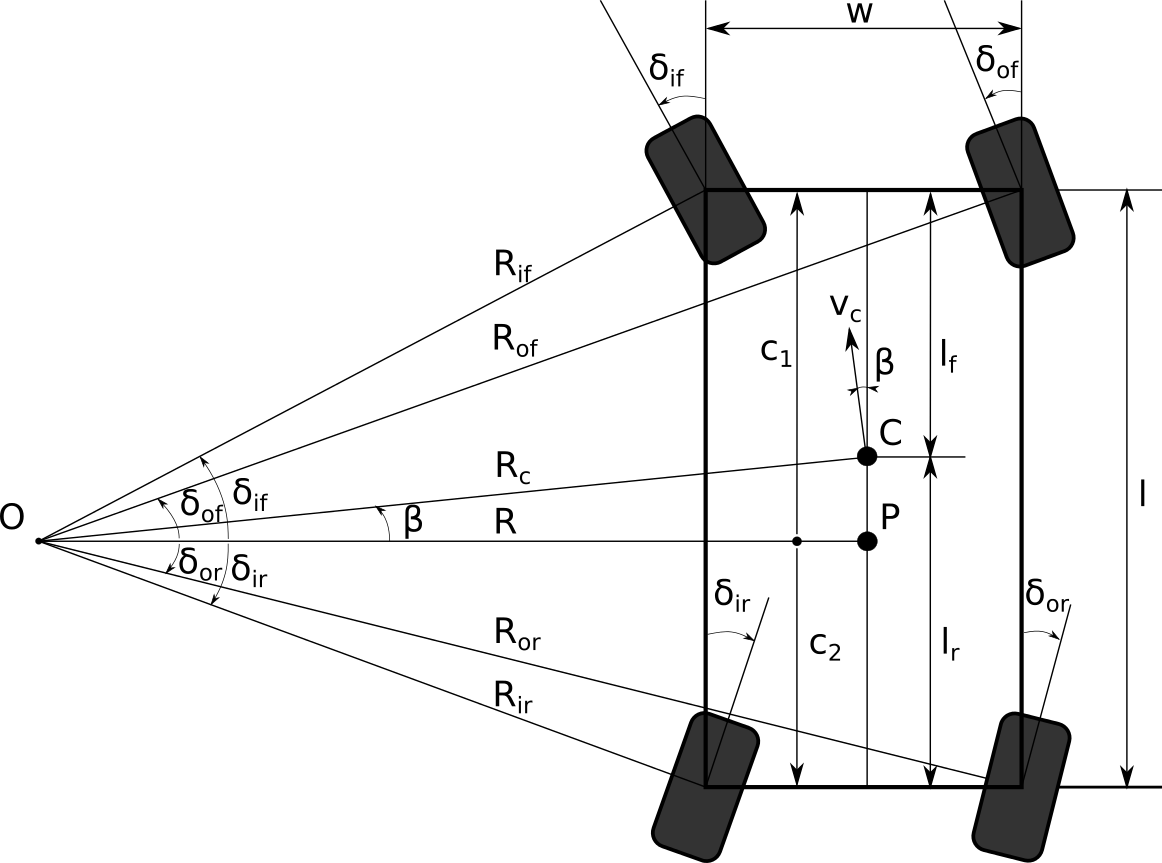
\includegraphics[width=0.7\linewidth]{Chapters/Chapter2/Figures/4ws_model.png}
	\caption{Κινηματικό μοντέλο αρνητικής τετραδιεύθυνσης.}
	\label{fig:4ws_model}
\end{figure}

\begin{figure}[!ht]
	\centering
	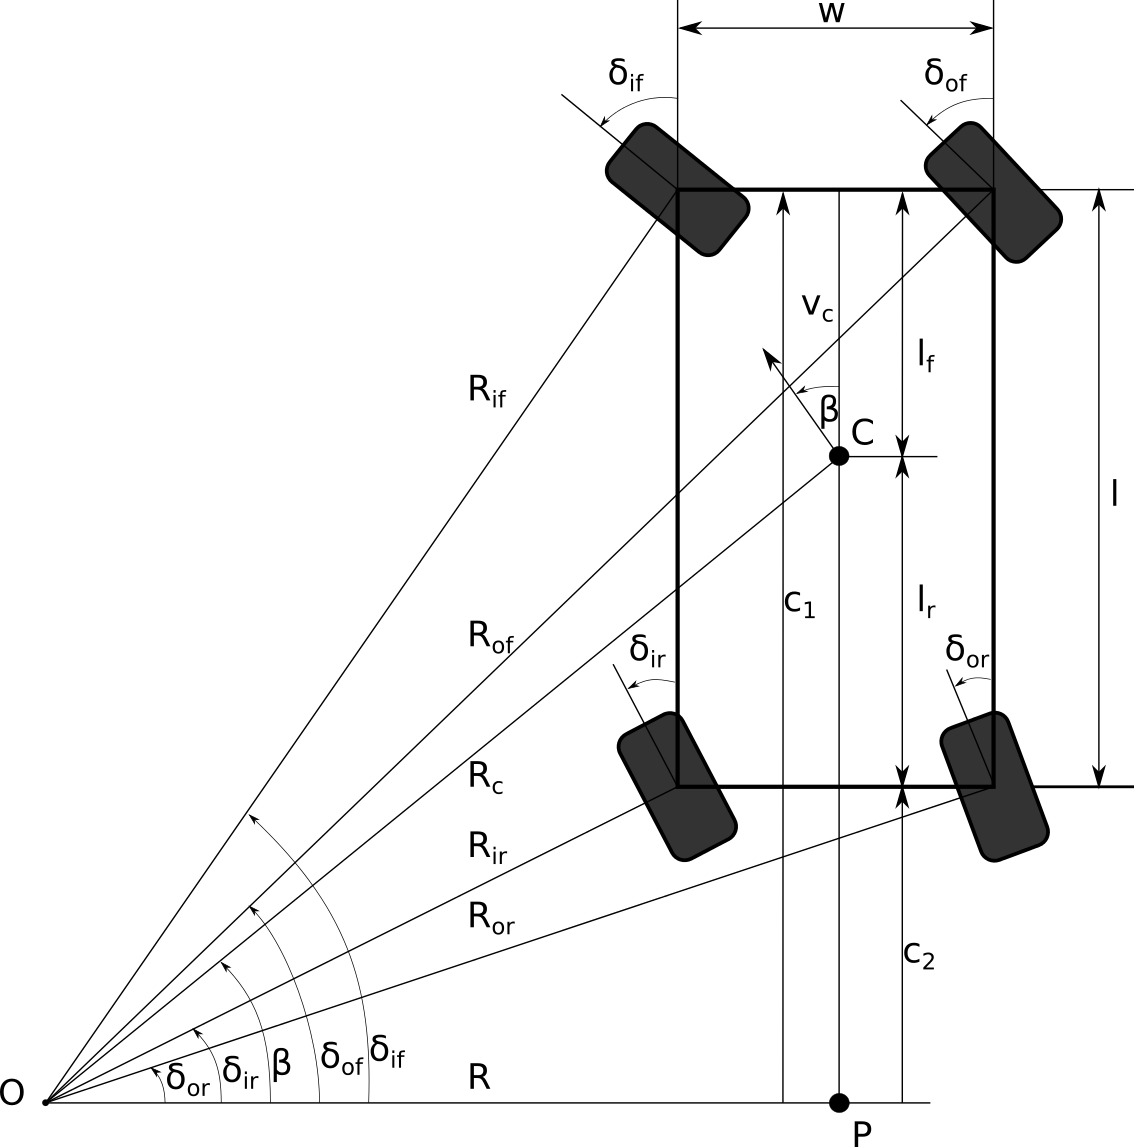
\includegraphics[width=0.7\linewidth]{Chapters/Chapter2/Figures/pos_4ws_model.png}
	\caption{Κινηματικό μοντέλο θετικής τετραδιεύθυνσης.}
	\label{fig:pos_4ws_model}
\end{figure}

\bigskip
Μέσω γεωμετρικής ανάλυσης του σχήματος \ref{fig:4ws_model}, βάση του ορισμού της \textit{συνθήκης τετραδιεύθυνσης}, προκύπτουν οι γωνίες στρέψης των τροχών του οχήματος:

\begin{align}
	\tan{\delta_{if}} &= \frac{c_1}{R-\frac{w}{2}}
	\label{eq:4ws_front_inner_steering_angle}\\
	\tan{\delta_{of}} &= \frac{c_1}{R+\frac{w}{2}}
	\label{eq:4ws_front_outer_steering_angle}\\
	\tan{\delta_{ir}} &= \frac{c_2}{R-\frac{w}{2}}
	\label{eq:4ws_rear_inner_steering_angle}\\
	\tan{\delta_{or}} &= \frac{c_2}{R+\frac{w}{2}}
	\label{eq:4ws_rear_outer_steering_angle}		
\end{align}

Aντιστρέφοντας και αφαιρώντας τις σχέσεις (\ref{eq:4ws_front_inner_steering_angle}), (\ref{eq:4ws_front_outer_steering_angle}) και (\ref{eq:4ws_rear_inner_steering_angle}), (\ref{eq:4ws_rear_outer_steering_angle}) προκύπτουν οι συνθήκες τετραδιεύθυνσης των μπροστινών και πίσω τροχών, αντίστοιχα.

\begin{align}
	\cot{\delta_{of}} - \cot{\delta_{if}} &= \frac{w}{c_1}
	\label{eq:front_4ws_condition}\\
	\cot{\delta_{or}} - \cot{\delta_{ir}} &= \frac{w}{c_2}
	\label{eq:rear_4ws_condition}
\end{align}

\noindent
Έπειτα, προσθέτοντας τις προκύπτουσες εξισώσεις (\ref{eq:front_4ws_condition}), (\ref{eq:rear_4ws_condition}), λαμβάνεται η μαθηματική εξίσωση της \textit{συνθήκης τετραδιεύθυνσης}.

\begin{equation}
	\frac{1}{\cot{\delta_{of}} - \cot{\delta_{if}}} + \frac{1}{\cot{\delta_{or}} - \cot{\delta_{ir}}} = \frac{c_1 - c_2}{w} = \frac{l}{w}
	\label{eq:4ws_condition}
\end{equation}


\bigskip\bigskip
H γωνία $\beta$ πλευρικής ολίσθησης (sideslip angle) \cite{automated_odometry} του κέντρου μάζας $\,C\,$ του οχήματος, υπολογίζεται, εύκολα, από το ισοδύναμο \textit{μοντέλο ποδηλάτου τετραδιεύθυνσης} (σχήμα \ref{fig:4ws_bicycle}).

\begin{equation}
	\tan{\beta} = \frac{l_r \cdot \tan{\delta_f} + l_f \cdot \tan{\delta_r}}{l}
	\label{eq:neg_4ws_beta}\\
\end{equation} 

\noindent
όπου
\begin{description}
	\item[\delta_f:] γωνία στρέψης μπροστινού τροχού ισοδύναμου μοντέλου ποδηλάτου τετραδιεύθυνσης
	\item[\delta_r:] γωνία στρέψης πίσω τροχού ισοδύναμου μοντέλου ποδηλάτου τετραδιεύθυνσης
\end{description}

\bigskip
Οι γωνίες στρέψης $\delta_f$ και $\delta_r$, μπορούν να υπολογιστούν για ένα όχημα με \textit{τετραδιεύθυνση} ως

\begin{align}
	\cot{\delta_f} &= \frac{\cot{\delta_{if}} + \cot{\delta_{of}}}{2} = \frac{R}{c_1}
	\label{eq:df}\\
	\cot{\delta_r} &= \frac{\cot{\delta_{ir}} + \cot{\delta_{or}}}{2} = \frac{R}{c_2}
	\label{eq:dr}
\end{align}

\bigskip
Αντιστρέφοντας και αφαιρώντας τις εξισώσεις (\ref{eq:dr}), (\ref{eq:df}), υπολογίζεται η ακτίνα $R$ της τροχιά, του σημείου $P$

\begin{equation}
	R = \frac{l}{\tan{\delta_f} - \tan{\delta_r}}
	\label{eq:pos_p_turning_radius}
\end{equation}


\bigskip
\noindent
και έπειτα η ακτίνα $R_c$ της τροχιάς του κέντρου μάζας $C$ του οχήματος.

\begin{equation}
	R_c = \frac{R}{\cos{\beta}} = \frac{l}{\cos{\beta} \cdot (\tan{\delta_f} - \tan{\delta_r})}
\end{equation}

\begin{figure}[!ht]
	\centering
	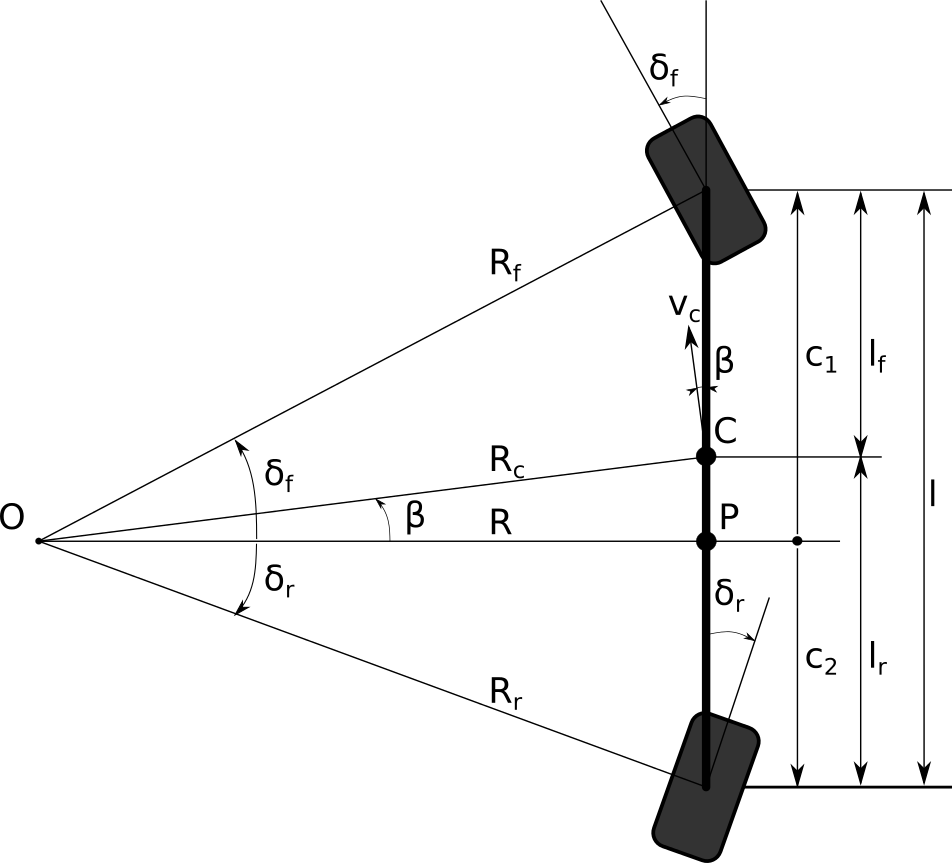
\includegraphics[width=0.6\linewidth]{Chapters/Chapter2/Figures/4ws_bicycle.png}
	\caption{Ισοδύναμο μοντέλο ποδηλάτου αρνητικής τετραδιεύθυνσης.}
	\label{fig:4ws_bicycle}
\end{figure}

\begin{figure}[!ht]
	\centering
	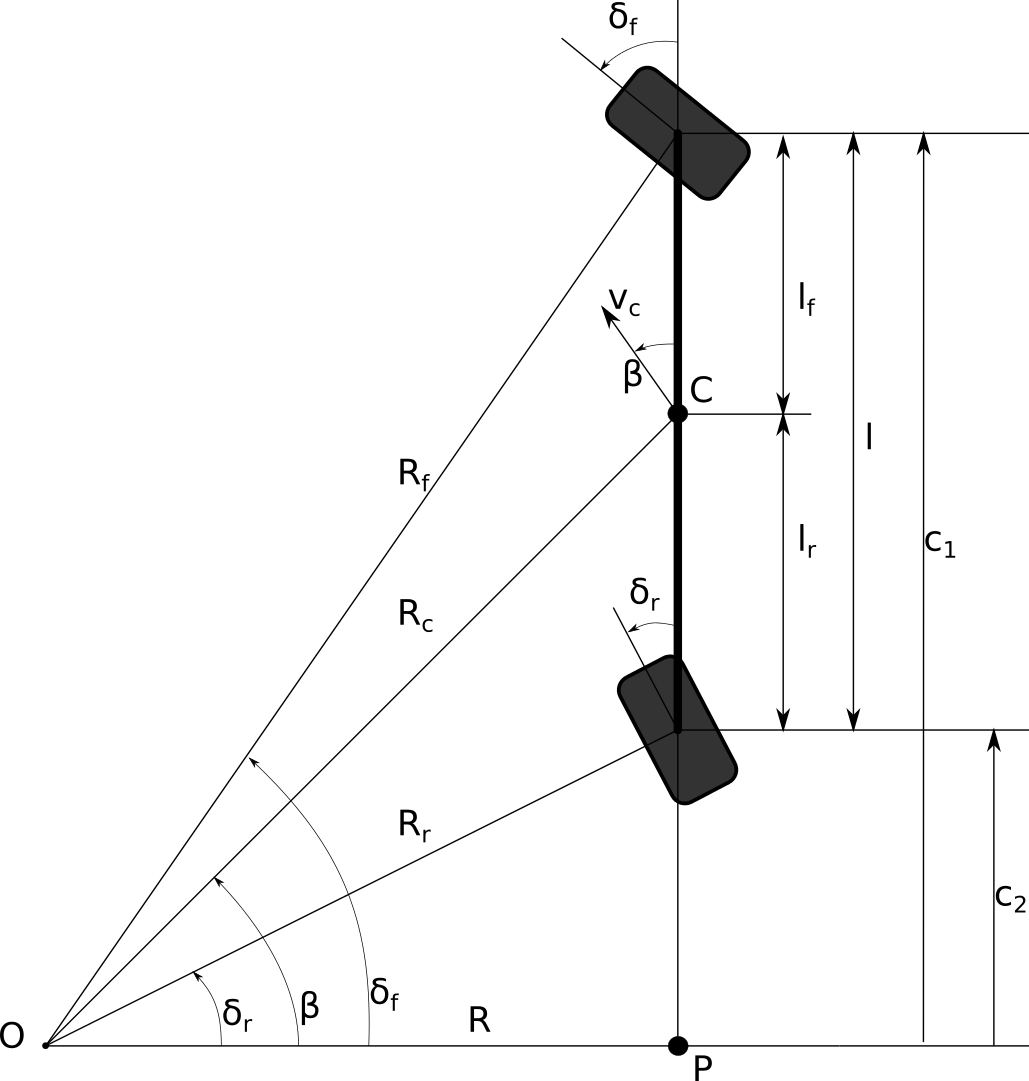
\includegraphics[width=0.6\linewidth]{Chapters/Chapter2/Figures/pos_4ws_bicycle_model.png}
	\caption{Ισοδύναμο μοντέλο ποδηλάτου θετικής τετραδιεύθυνσης.}
	\label{fig:pos_4ws_bicycle_model}
\end{figure}



%\bigskip
%Για δεδομένη επιθυμητή τροχιά, ακτίνας R, του οχήματος, οι εξισώσεις (\ref{eq:4ws_front_inner_steering_angle})-(\ref{eq:4ws_rear_outer_steering_angle}) έχουν παραπάνω από μία λύση, γεγονός που περιπλέκει σημαντικά τους υπολογισμούς. Για την απλοποίηση του προβλήματος χρησιμοποιείται μία υποπερίπτωση του κινηματικού μοντέλου (σχήμα \ref{fig:4ws_simplified_model}), με βάση την οποία το κέντρο μάζας $C$ του οχήματος ταυτίζεται με το σημείο P, το οποίο αποτελεί το σημείο τομής του επιμήκη άξονα του οχήματος με την ευθεία που διέρχεται κάθετα από αυτόν και τον ενώνει με το \textit{Στιγμιαίο Κέντρο Περιστροφής Ο}. Σαν αποτέλεσμα, ισχύουν τα εξής:
%
%\begin{align}
%	\begin{split}
%		c_1 &= l_f\\
%		c_2 &= l_r\\
%		\beta &= 0^\circ
%	\end{split}
%	\label{eq:simple_4ws_conditions}
%\end{align}
%
%\begin{figure}[!ht]
%	\centering
%	\includegraphics[width=0.7\linewidth]{Chapters/Chapter2/Figures/4ws_simplified_model.png}
%	\caption{Κινηματικό μοντέλο απλοποιημένης αρνητικής τετραδιεύθυνσης.}
%	\label{fig:4ws_simplified_model}
%\end{figure}
%
%\bigskip
%Οπότε οι σχέσεις (\ref{eq:4ws_front_inner_steering_angle})-(\ref{eq:4ws_rear_outer_steering_angle}), με βάση τις συνθήκες (\ref{eq:simple_4ws_conditions}) μετασχηματίζονται στην ακόλουθη μορφή:
%
%
%\begin{align}
%	\tan{\delta_{if}} &= \frac{l_f}{R-\frac{w}{2}}
%	\label{eq:4ws_simple_front_inner_steering_angle}\\
%	\tan{\delta_{of}} &= \frac{l_f}{R+\frac{w}{2}}
%	\label{eq:4ws_simple_front_outer_steering_angle}\\
%	\tan{\delta_{ir}} &= \frac{l_r}{R-\frac{w}{2}}
%	\label{eq:4ws_simple_rear_inner_steering_angle}\\
%	\tan{\delta_{or}} &= \frac{l_r}{R+\frac{w}{2}}
%	\label{eq:4ws_simple_rear_outer_steering_angle}		
%\end{align}

\bigskip
Για τον υπολογισμό των ταχυτήτων θα χρησιμοποιηθούν και πάλι, οι εξισώσεις (\ref{eq:theta_dot})-(\ref{eq:theta_dot_2}), εφόσον ισχύουν και στην προκειμένη περίπτωση, σε συνδυασμό με τις σχέσεις των ακτίνων τροχιάς κάθε τροχού, όπως προκύπτει από το σχήμα \ref{fig:4ws_model}.

\begin{align}
	R_{if} &= \frac{R - \frac{w}{2}}{\cos{\delta_{if}}}
	\label{eq:neg_4ws_rif}\\
	R_{of} &= \frac{R + \frac{w}{2}}{\cos{\delta_{of}}}
	\label{eq:neg_4ws_rof}\\
	R_{ir} &= \frac{R - \frac{w}{2}}{\cos{\delta_{ir}}}
	\label{eq:neg_4ws_rir}\\
	R_{or} &= \frac{R + \frac{w}{2}}{\cos{\delta_{or}}}
	\label{eq:neg_4ws_or}
\end{align}

\bigskip
Επομένως, οι γραμμικές ταχύτητες των τροχών προκύπτουν, ως

\begin{align}
	\label{eq:neg_4ws_vif}	
	v_{if} &= \dot\theta \cdot R_{if} = \frac{v_c}{R_c} \cdot \frac{R - \frac{w}{2}}{\cos{\delta_{if}}}\\
	\label{eq:neg_4ws_vof}	
	v_{of} &= \dot\theta \cdot R_{of} = \frac{v_c}{R_c} \cdot \frac{R + \frac{w}{2}}{\cos{\delta_{of}}}\\
	\label{eq:neg_4ws_vir}	
	v_{ir} &= \dot\theta \cdot R_{ir} = \frac{v_c}{R_c} \cdot \frac{R - \frac{w}{2}}{\cos{\delta_{ir}}} \\
	\label{eq:neg_4ws_vor}
	v_{or} &= \dot\theta \cdot R_{or} = \frac{v_c}{R_c} \cdot \frac{R + \frac{w}{2}}{\cos{\delta_{or}}}
\end{align}

\bigskip
\noindent
και αντίστοιχα οι περιστροφικές ταχύτητες των τροχών, με βάση την εξίσωση (\ref{eq:v_omega}), προκύπτουν

\begin{align}
	\label{eq:neg_4ws_wif}	
	\omega_{if} &= \frac{v_{if}}{r} = \frac{v_c}{r \cdot R_c} \cdot \frac{R - \frac{w}{2}}{\cos{\delta_{if}}}\\
	\label{eq:neg_4ws_wof}	
	\omega_{of} &= \frac{v_{if}}{r} = \frac{v_c}{r \cdot R_c} \cdot \frac{R + \frac{w}{2}}{\cos{\delta_{of}}}\\
	\label{eq:neg_4ws_wir}	
	\omega_{ir} &= \frac{v_{if}}{r} = \frac{v_c}{r \cdot R_c} \cdot \frac{R - \frac{w}{2}}{\cos{\delta_{ir}}} \\
	\label{eq:neg_4ws_wor}
	\omega_{or} &= \frac{v_{if}}{r} = \frac{v_c}{r \cdot R_c} \cdot \frac{R + \frac{w}{2}}{\cos{\delta_{or}}}
\end{align} 

\bigskip
Με βάση την παραπάνω κινηματική ανάλυση, οι εξισώσεις των ταχυτήτων, του οχήματος, ως προς το κέντρο μάζας του \textit{C}, μπορούν να υπολογιστούν, χρησιμοποιώντας τις σχέσεις

\begin{equation}
	\tan{\beta} = \frac{v_{c,y}}{v_{c,x}} \;\;\Leftrightarrow\;\; v_{c,y} = v_{c,x} \cdot \tan{\beta}
	\label{eq:vel_beta}
\end{equation}
\begin{equation}
	v_c^2 = v_{c,x}^2 + v_{c,y}^2 \;\;\Leftrightarrow\;\; v_{c}^2 = v_{c,x}^2 - v_{c,x}^2  \cdot \tan^2{\beta}
	\label{eq:v_squared}
\end{equation}
\begin{equation}
	v_c = \omega_c \cdot R_c
	\label{eq:lin_ang_relationship}
\end{equation}

\noindent
από τις οποίες, τελικά προκύπτουν οι εξισώσεις των ταχυτήτων του οχήματος, ως προς το κέντρο μάζας του $C$:

\begin{align}
	v_{c,x} &= \frac{v_c}{\sqrt{1+\tan^2\beta}}
	\label{eq:lin_vel_x}\\
	v_{c,y} &= \frac{v_c \cdot \tan{\beta}}{\sqrt{1+\tan^2\beta}}
	\label{eq:lin_vel_y}\\
	\omega_c &= \frac{v_c \cdot \cos{\beta} \cdot (\tan{\delta_f - \tan{\delta_r}})}{l}
	\label{eq:ang_vel}
\end{align}

\bigskip\noindent
όπου
\begin{description}
	\item[v_c:] η συνισταμένη γραμμική ταχύτητα του κέντρου μάζας του οχήματος
	\item[v_{c,x}:] η γραμμική επιμήκης ταχύτητα του κέντρου μάζας του οχήματος
	\item[v_{c,y}:] η γραμμική εγκάρσια ταχύτητα του κέντρου μάζας του οχήματος
	\item[\omega_c:] η γωνιακή ταχύτητα του κέντρου μάζας του οχήματος
\end{description}

\bigskip\bigskip
Τέλος, οι ταχύτητες κέντρου μάζας $C$ του οχήματος, ως προς ένα αυθαίρετο εξωτερικό σύστημα συντεταγμένων, προκύπτουν βάση του \textit{ισοδύναμου κινηματικού μοντέλου ποδηλάτου τετραδιεύθυνσης} (σχήμα \ref{fig:4ws_bicycle}) \cite{4ws_trajectory_planning}.

\begin{align}
	\dot X &= v_c \cdot \cos(\theta + \beta)
	\label{eq:x_dot}\\
	\dot Y &= v_c \cdot \sin(\theta + \beta)
	\label{eq:y_dot}\\
	\dot \Theta &= \omega_c = \frac{v_c \cdot \cos{\beta} \cdot (\tan{\delta_f - \tan{\delta_r}})}{l}
	\label{eq:th_dot}
\end{align}

\noindent
όπου,
\begin{equation}
	v_c = \frac{v_f \cdot \cos{\delta_f} + v_r \cos{\delta_r}}{2 \cdot \cos{\beta}}
	\label{eq:v_c_f_r}
\end{equation}

\begin{figure}[!ht]
	\centering
	\includegraphics[width=0.6\linewidth]{Chapters/Chapter2/Figures/4ws_xy_plane.png}
	\caption[Ισοδύναμο κινηματικό μοντέλο ποδηλάτου τετραδιεύθυνσης στο επίπεδο ΧΥ.]{Ισοδύναμο κινηματικό μοντέλο ποδηλάτου τετραδιεύθυνσης στο επίπεδο ΧΥ \cite{4ws_trajectory_planning}.}
	\label{fig:4ws_xy_plane}
\end{figure}

%%%%%%%%%%%%%%%%%%%%%%%%%%%%%%%%%%%%%%%%%%%%%%%%%%%%%%%%%%%%%%%%%%%%%%%%%%%%%%%%%%%%%%%%%%%%%%
%%%%%%%%%%%%%%%%%%%%%%%%%%%%%%%%%%%%%%%%%%%%%%%%%%%%%%%%%%%%%%%%%%%%%%%%%%%%%%%%%%%%%%%%%%%%%%
\newpage
\bigskip
\subsection{Κινηματικό Μοντέλο Ρομποτικής Πλατφόρμας \textit{Monstertruck}} \label{ssec:monstertruck_kinematics}
Η ρομποτική πλατφόρμα \textit{Monstertruck} περιλαμβάνει ένα \textit{μη ιδανικό κινηματικό μοντέλο τετραδιεύθυνσης}, με την έννοια, ότι δεν υπακούει στην \textit{συνθήκη τετραδιεύθυνσης} (\ref{eq:4ws_condition}). Το γεγονός αυτό, οφείλεται στο μηχανισμό μετάδοσης της στρέψης των τροχών που παρουσιάστηκε στην ενότητα \ref{ssec:four_wheel_steering} και ο οποίος ορίζει μία σχέση, μεταξύ εσωτερικού και εξωτερικού τροχού, με αρκετά μεγάλη απόκλιση από την ιδανική συνθήκη τετραδιεύθυνσης \ref{eq:4ws_condition}, ή ακόμα και από την ιδανική συνθήκη Ackermann \ref{eq:ackermann_condition} όπως παρουσιάζεται και στο σχήμα \ref{fig:steer_angles_comparison}.

\begin{figure}[!ht]
	\centering
	\includegraphics[width=0.6\linewidth]{Chapters/Chapter2/Figures/steer_angles_comparison.png}
	\caption{Η σχέση στρέψης μεταξύ εσωτερικού και εξωτερικού τροχού για τα κινηματικά μοντέλα \\Ackermann, Τετραδιεύθυνσης και της ρομποτικής πλατφόρμας Monstertruck.}
	\label{fig:steer_angles_comparison}
\end{figure}

Εφόσον, παραβιάζεται η \textit{συνθήκη τετραδιεύθυνσης} (\ref{eq:4ws_condition}), η κίνηση της ρομποτικής πλατφόρμας \textit{Monstertruck}, θα επιβαρύνεται από πλευρική ολίσθηση των τροχών. Παρόλα αυτά, επειδή, η ρομποτική πλατφόρμα, σχεδιάστηκε και προορίζεται για εφαρμογές εξαιρετικά μικρών ταχυτήτων και επομένως τυχόν δυναμικά φαινόμενα, που παρουσιάζονται, κατά την κίνηση, είναι αμελητέα, η κίνηση της ρομποτικής πλατφόρμας, μπορεί να προσεγγισθεί από το \textit{ιδανικό κινηματικό μοντέλο τετραδιεύθυνσης}. 

\bigskip
Για την κινηματική ανάλυση του μοντέλου της ρομποτικής πλατφόρμας \textit{Monstertruck}, θα χρησιμοποιήσουμε τις παραδοχές, ότι η διαφορά της γωνίας στρέψης μεταξύ δεξιού και αριστερού τροχού είναι αμελητέα και ότι σε χαμηλές ταχύτητες, η κίνηση της ρομποτικής πλατφόρμας, περιγράφεται, με αμελητέο σφάλμα, από τις εξισώσεις κίνησης του κινηματικού μοντέλου \textit{τετραδιεύθυνσης} στο επίπεδο.

%Θα χρησιμοποιήσουμε το \textit{ισοδύναμο κινηματικό μοντέλο ποδηλάτου τετραδιεύθυνσης} (σχήματα \ref{fig:4ws_bicycle}, \ref{fig:pos_4ws_bicycle_model}) και τις εξισώσεις ταχυτήτων του οχήματος (\ref{eq:lin_vel_x} - \ref{eq:ang_vel}, \ref{eq:v_c_f_r})  για να εξάγουμε, έπειτα, τις εξισώσεις στρέψης και ταχύτητας των τροχών (αντίστροφη κινηματική ανάλυση).

\bigskip
Το \textit{μη ιδανικό κινηματικό μοντέλο τετραδιεύθυνσης} της ρομποτικής πλατφόρμας \textit{Monstertruck}, παρουσιάζεται στο σχήμα \ref{fig:monstetruck_model}. Στο μοντέλο αυτό, το \textit{Στιγμιαίο Κέντρο Περιστροφής Ο}, βρίσκεται στην τομή των κάθετων στους τροχούς, αξόνων του \textit{ισοδύναμου κινηματικού μοντέλου ποδηλάτου τετραδιεύθυνσης}. Σαν αποτέλεσμα η διεύθυνση κάθε τροχού είναι διάφορη της διεύθυνσης της ταχύτητας του κατά μία γωνία $\alpha$, που ονομάζεται \textit{γωνία πλευρικής ολίσθησης τροχού (side slip angle)} \cite{4ws_kinematics}, όπως παρουσιάζεται στο σχήμα \ref{fig:monstertruck_slip_angle_model}.


\begin{figure}[!ht]
	\centering
	\includegraphics[width=0.7\linewidth]{Chapters/Chapter2/Figures/monstertruck_model_parallel.png}
	\caption{Το κινηματικό μοντέλο της ρομποτικής πλατφόρμας Monstertruck,\\ σε διάταξη αρνητικής τετραδιεύθυνσης.}
	\label{fig:monstetruck_model}
\end{figure}

\bigskip
Με βάση το μη ιδανικό μοντέλο τετραδιεύθυνσης, που παρουσιάζεται στο σχήμα \ref{fig:monstertruck_slip_angle_model}, ο εσωτερικός τροχός στρέφεται κατά ίδια γωνία με τον αντίστοιχο εξωτερικό. Παρόλα αυτά, επειδή το όχημα, εκτελεί μία περιστροφική κίνηση, γύρω από το $O$, οι εξωτερικοί τροχοί διανύουν μεγαλύτερη απόσταση από τους εσωτερικούς, το οποίο σημαίνει ότι οι τροχοί ολισθαίνουν. Οι γωνίες της συνισταμένης ταχύτητας των τροχών δίνονται από τις ακόλουθες σχέσεις.

\begin{align}
	\cot(\delta_{if} + \alpha_{if}) = \frac{R - \frac{w}{2}}{c_1}
	\label{eq:monst_dif}\\
	\cot(\delta_{of} - \alpha_{of}) = \frac{R + \frac{w}{2}}{c_1}
	\label{eq:monst_dof}\\
	\cot(\delta_{ir} + \alpha_{ir}) = \frac{R - \frac{w}{2}}{c_2} 
	\label{eq:monst_dir}\\
	\cot(\delta_{or} - \alpha_{or}) = \frac{R + \frac{w}{2}}{c_2}
	\label{eq:monst_dor}
\end{align}


\begin{figure}[!ht]
	\centering
	\includegraphics[width=0.7\linewidth]{Chapters/Chapter2/Figures/monstertruck_slip_angle_model_parallel.png}
	\caption{Το μη ιδανικό κινηματικό μοντέλο τετραδιεύθυνσης, με πλευρική ολίσθηση τροχών,\\ της ρομποτικής πλατφόρμας Monstertruck, σε διάταξη αρνητικής τετραδιεύθυνσης.}
	\label{fig:monstertruck_slip_angle_model}
\end{figure}

\bigskip
Αφαιρώντας τις (\ref{eq:monst_dif}), (\ref{eq:monst_dof}) και (\ref{eq:monst_dif}), (\ref{eq:monst_dof}) προκύπτουν οι σχέσεις τετραδιεύθυνσης του μη ιδανικού μοντέλου, για τους μπροστινούς και πίσω τροχούς.

\begin{align}
	\cot(\delta_{of} - \alpha_{of}) - \cot(\delta_{if} + \alpha_{if}) = \frac{w}{c1}
	\label{eq:monst_front_condition}\\
	\cot(\delta_{or} - \alpha_{or}) - \cot(\delta_{ir} + \alpha_{ir}) = \frac{w}{c2}
	\label{eq:monst_rear_condition}\\
\end{align}

\bigskip
Έπειτα, αντιστρέφοντας και αφαιρώντας τις σχέσεις (\ref{eq:monst_front_condition}), (\ref{eq:monst_rear_condition}) προκύπτει τελικά, η \textit{κινηματική συνθήκη του μη ιδανικού μοντέλου τετραδιεύθυνσης της ρομποτικής πλατφόρμας Monstertruck} \cite{4ws_kinematics}. 

\begin{equation}
	\frac{1}{\cot(\delta_{of} - \alpha_{of}) - \cot(\delta_{if} + \alpha_{if})} - \frac{1}{\cot(\delta_{or} - \alpha_{or}) - \cot(\delta_{ir} + \alpha_{ir})} = \frac{c_1 - c_2}{w} = \frac{l}{w}
	\label{eq:monst_kinematic_condition}
\end{equation}

\bigskip
Με βάση την παραδοχή, ότι το όχημα περιστρέφεται με συνισταμένη γραμμική ταχύτητα $v_c$ και γωνιακή ταχύτητα $\omega_c$, γύρω από το κέντρο $O$, υπολογίζονται αρχικά οι ακτίνες περιστροφής των τροχών γύρω από το κέντρο $O$.

\begin{align}
	R_{if} = \frac{R_c}{\cos(\delta_{if} + \alpha_{if})}
	\label{eq:monst_rif}\\
	R_{of} = \frac{R_c}{\cos(\delta_{of} - \alpha_{of})}
	\label{eq:monst_rof}\\
	R_{ir} = \frac{R_c}{\cos(\delta_{ir} + \alpha_{ir})}
	\label{eq:monst_rir}\\
	R_{or} = \frac{R_c}{\cos(\delta_{or} - \alpha_{or})}
	\label{eq:monst_ror}
\end{align}

\bigskip
Έπειτα, μπορούμε να υπολογίσουμε τις συνισταμένες ταχύτητες κάθε τροχού γύρω από το κέντρο $O$, χρησιμοποιώντας την αντίστοιχη ακτίνα τροχιάς.

\begin{align}
	\label{eq:monst_vif}	
	v_{if} &= \dot\theta \cdot R_{if} = \frac{v_c}{R_c} \cdot \frac{R - \frac{w}{2}}{\cos(\delta_{if} - \alpha_{if})}\\
	\label{eq:monst_vof}	
	v_{of} &= \dot\theta \cdot R_{of} = \frac{v_c}{R_c} \cdot \frac{R + \frac{w}{2}}{\cos(\delta_{of} - \alpha_{of})}\\
	\label{eq:monst_vir}	
	v_{ir} &= \dot\theta \cdot R_{ir} = \frac{v_c}{R_c} \cdot \frac{R - \frac{w}{2}}{\cos(\delta_{ir} + \alpha_{ir})} \\
	\label{eq:monst_vor}
	v_{or} &= \dot\theta \cdot R_{or} = \frac{v_c}{R_c} \cdot \frac{R + \frac{w}{2}}{\cos(\delta_{or} - \alpha_{or})}
\end{align}

Επομένως, με βάση τις συνισταμένες ταχύτητες $v$ και τις γωνίες πλευρικής ολίσθησης $\alpha$, (σχήμα \ref{fig:slip_angles})μπορούμε να υπολογίσουμε τις επιμήκεις ταχύτητες των τροχών ως

\begin{align}
	\label{eq:monst_vifx}	
	v_{if,x} &= \frac{v_{if}}{\cos\alpha_{if}}\\
	\label{eq:monst_vofx}	
	v_{of,x} &= \frac{v_{of}}{\cos\alpha_{of}} \\
	\label{eq:monst_virx}	
	v_{ir,x} &= \frac{v_{ir}}{\cos\alpha_{ir}} \\
	\label{eq:monst_vorx}
	v_{or,x} &= \frac{v_{or}}{\cos\alpha_{or}}
\end{align}

\begin{figure}[!ht]
   \centering
	\includegraphics[width=0.4\linewidth]{Chapters/Chapter2/Figures/slip_angles.png}
	\caption{Ολίσθηση τροχών, λόγω μη ιδανικού μηχανισμού στρέψης.}
	\label{fig:slip_angles}
\end{figure}


\bigskip
Τέλος, οι περιστροφικές ταχύτητες των τροχών, υπολογίζονται από τις ακόλουθες σχέσεις

\begin{align}
	\label{eq:monst_wif}	
	\omega_{if} &= \frac{v_{if,x}}{r} = \frac{v_c \cdot (R - \frac{w}{2})}{r \cdot R_c \cdot \cos\alpha_{if} \cdot \cos(\delta_{if} - \alpha_{if})}\\
	\label{eq:monst_wof}
	\omega_{of} &= \frac{v_{of,x}}{r} = \frac{v_c \cdot (R + \frac{w}{2})}{r \cdot R_c \cdot \cos\alpha_{of} \cdot \cos(\delta_{of} - \alpha_{of})}\\
	\label{eq:monst_wir}	
	\omega_{ir} &= \frac{v_{ir,x}}{r} = \frac{v_c \cdot (R - \frac{w}{2})}{r \cdot R_c \cdot \cos\alpha_{ir} \cdot \cos(\delta_{ir} - \alpha_{ir})}\\
	\label{eq:monst_wor}
	\omega_{or} &= \frac{v_{or,x}}{r} = \frac{v_c \cdot (R + \frac{w}{2})}{r \cdot R_c \cdot \cos\alpha_{or} \cdot \cos(\delta_{or} - \alpha_{or})}
\end{align}

\bigskip
Οι παραπάνω τύποι, μπορούν να χρησιμοποιηθούν και για διαφορετικά κινηματικά μοντέλα \textit{τετραδιεύθυνσης}, αντικαθιστώντας κατάλληλα τις γωνίες στρέψης $\delta$ και τις γωνίες πλευρικής ολίσθησης $\alpha$. Επίσης, περιγράφουν και το ιδανικό κινηματικό μοντέλο \textit{τετραδιεύθυνσης} για μηδενικές γωνίες πλευρικής ολίσθησης $\alpha$ των τροχών και για γωνίες στρέψης $\delta$ που υπακούν στις εξισώσεις  (\ref{eq:4ws_front_inner_steering_angle})-(\ref{eq:4ws_rear_outer_steering_angle}).

\bigskip
Για τις γωνίες στρέψης της ρομποτικής πλατφόρμας Monstertruck, με βάση την παραδοχή της αμελητέας διαφοράς στρέψης, ισχύουν οι ακόλουθες εξισώσεις.

\begin{align}
	\delta_{if} = \delta_{of} = \delta_{f}
	\label{eq:monst_front_angles}\\
	\delta_{ir} = \delta_{or} = \delta_{r}
	\label{eq:monst_rear_angles}
\end{align}

Επομένως, οι γωνίες πλευρικής ολίσθησης των τροχών προκύπτουν ως

\begin{align}
	\alpha_{if} &= \tan^{-1}(\frac{c_1}{R-\frac{w}{2}}) - \delta_f
	\label{eq:monst_aif}\\
	\alpha_{of} &= -\tan^{-1}(\frac{c_1}{R+\frac{w}{2}}) + \delta_f
	\label{eq:monst_aof}\\
	\alpha_{ir} &= \tan^{-1}(\frac{c_2}{R-\frac{w}{2}}) - \delta_r
	\label{eq:monst_air}\\
	\alpha_{or} &= -\tan^{-1}(\frac{c_2}{R+\frac{w}{2}}) + \delta_r
	\label{eq:monst_aor}	
\end{align}


Τέλος, οι ταχύτητες του κέντρου μάζας C του οχήματος, ως προς ένα αυθαίρετο σύστημα συντεταγμένων, υπολογίζονται από τους τύπους του ιδανικού κινηματικού μοντέλου τετραδιεύθυνσης (\ref{eq:x_dot})-(\ref{eq:th_dot}).

